\documentclass[a4paper,12pt,twoside]{report}

\usepackage{acronym}
\usepackage{url}
\usepackage{cite}
\usepackage{listings}
\usepackage[pdftex]{graphicx}
\usepackage[hang,small,bf]{caption}
\usepackage{styles/tum}
\usepackage{setspace}
\usepackage[german,english]{babel}
\usepackage{float}
\usepackage{floatflt}
\usepackage{fancyhdr}
\usepackage{color}
\usepackage{booktabs}
\usepackage[pdftex,bookmarks=true,plainpages=false,pdfpagelabels=true]{hyperref}
\usepackage{mdwlist}
\usepackage{enumerate}
\usepackage{paralist}
\usepackage{array}
\usepackage{longtable}
\usepackage{amsmath}
\usepackage{algorithm}
\usepackage[noend]{algpseudocode}
\usepackage{listings}
\usepackage[utf8]{inputenc}
\usepackage[capitalize, noabbrev]{cleveref}
\usepackage{mathtools}
\usepackage{subcaption}
\usepackage{multirow}
\DeclarePairedDelimiter{\ceil}{\lceil}{\rceil}

\makeatletter
\renewenvironment{abstract}{%
  \if@twocolumn
    \section*{\abstractname}%
  \else
    \small
    \begin{center}%
      {\bfseries \abstractname\vspace{-.1em}\vspace{\z@}}%
    \end{center}%
    \quotation
  \fi}
  {\if@twocolumn\else\endquotation\fi}
\makeatother

% Path for graphics
\graphicspath{{figures/}}

\begin{document}
\setlength{\evensidemargin}{22pt}
\setlength{\oddsidemargin}{22pt}

\def\doctype{Bachelor's Thesis}
\def\faculty{Informatics}
\def\title{Simulation-Based Analysis of Blockchain Architectures}		
\def\titleGer{Simulationsbasierte Analyse von Blockchain Architekturen}
\def\supervisor{Prof. Dr. Dr. h.c. Manfred Broy}
\def\advisor{Diego Marmsoler}
\def\author{Leo Eichhorn}
\def\date{13.07.2018}


\hypersetup{pdfborder={0 0 0},
                        pdfauthor={Leo Eichhorn},
                        pdftitle={Simulation-Based Analysis of Blockchain Architectures},
                        }

\lstset{showspaces=false, numbers=left, frame=single, basicstyle=\small}

%\pagenumbering{alph}


\thispagestyle{empty}

\vspace{4cm}
\begin{center}
\oTUM{4cm}\\ 
\vspace{5mm}     
\huge DEPARTMENT OF INFORMATICS\\ 
\vspace{0.5cm}
\large TECHNICAL UNIVERSITY OF MUNICH\\
\vspace{1mm}
\end{center}

\vspace{13mm}

\begin{center}
{\Large \doctype\ in \faculty}
\vspace{20mm}

\begin{spacing}{1.5}
{\huge\bf \title}\\%[3ex]
\end{spacing}

\vspace{15mm}
{\LARGE \author}

\vspace{10mm}

\begin{figure}[h!]
\centering
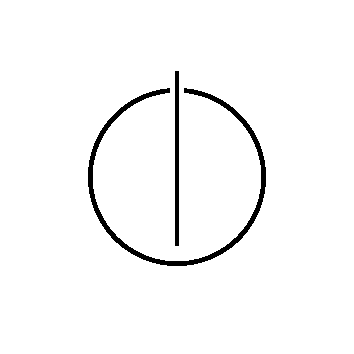
\includegraphics[width=4cm]{InformaticsLogo}
\end{figure}

\end{center}

\newpage
\thispagestyle{empty}
\mbox{}
\thispagestyle{empty}
\pagenumbering{roman}
\vspace{8mm}
\begin{center}
\oTUM{4cm}

\vspace{5mm}     
\huge DEPARTMENT OF INFORMATICS\\ 
\vspace{0.5cm}
\large TECHNICAL UNIVERSITY OF MUNICH\\
\end{center}

\vspace{5mm}

\begin{center}
{\Large \doctype\ in \faculty}
\vspace{8mm}

\begin{spacing}{1.3}
{\LARGE \title}\\
\vspace{8mm}

{\LARGE \titleGer}\\
\vspace{8mm}
\end{spacing}

\begin{tabular}{ll}
\Large Author:     & \Large \author     \\[2mm]
\Large Supervisor: & \Large \supervisor \\[2mm]				
\Large Advisor:	   & \Large \advisor    \\[2mm]
\Large Submission date:       & \Large \date
\end{tabular}

\vspace{1mm}

\begin{figure}[hb!]
\centering
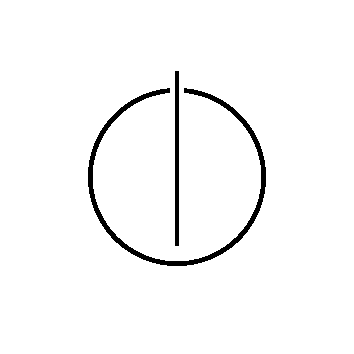
\includegraphics[width=4cm]{InformaticsLogo}
\end{figure}

\end{center}
\newpage
\thispagestyle{empty}
\mbox{}
\clearpage
\thispagestyle{empty}
\vspace*{0.8\textheight}
\noindent
I assure the single handed composition of this bachelor thesis only supported by declared resources,

\vspace{15mm}
\noindent
Munich, \date \hspace{\stretch{1}} \author
\newpage



\newpage
\thispagestyle{empty}
\mbox{}

\chapter*{Acknowledgements}
First of all, I would like to thank the chair for software and systems engineering and especially Prof. Manfred Broy for providing me with the opportunity of writing this thesis. Furthermore, I want to express my gratitude towards my advisor, Diego Marmsoler, for his guidance over the course of this project. His constructive feedback and helpful advice were invaluable to the completion of this work. Finally, I would like to thank my friends and family for their endless support and patience throughout my studies.
\clearpage
%\pagenumbering{roman}

\selectlanguage{english}
\begin{abstract}
A blockchain can be described a distributed database which is locally maintained and updated by a group of voluntary members. All participants of the architecture form a peer-to-peer network in order to broadcast and validate new data blocks to be included in the blockchain. Creating a block consists of cryptographically linking it to the previous block and computing a proof of work. By declaring the blockchain containing the most proof of work as the valid chain, only one version of the database can be accepted by all members. Because of the difficulty of calculating a valid proof of work, the blockchain is inherently resistant to the retroactive modification of its stored data. 

However, potential attacks against blockchain architectures enabling the modification of already confirmed blocks have been formulated, one of which is known as the \textit{double-spend attack.} This attack describes a group of dishonest nodes secretly mining new blocks on top of a modified block. After surpassing the proof of work contained in the honest chain, the secret branch is published and consequently accepted by the remaining network. 

The goal of this thesis is to empirically increase the understanding of factors affecting a blockchain architecture's resistance against these double-spend attacks. This is achieved by identifying a variety of potential factors influencing a blockchain's resistance and subsequently implementing them in a simulation of blockchain architectures. By conducting a range of experimental double-spend attacks on the simulated architecture, the effects of different parameter configurations are evaluated. Throughout our analysis we confirm that double-spend attacks are more likely at higher amounts of computing power controlled by the attacker and are only partially averted by a high number of confirmations. Additionally, we discover that especially the number of stale blocks created by the attacking and honest networks influences the amount of successful double-spend attacks. Stale blocks represent a natural branch of the main chain and are therefore not part of the valid blockchain. They consequently do not increase the blockchain's total proof of work and represent a waste of computing power in regards to averting or conducting double-spend attacks. We show that the amount of stale blocks is influenced by the rate at which new blocks are mined compared to the propagation delay caused by the network's topology and latency. Summarizing our results and data, we finally propose an empirical model of double-spend resistance representing the effects of all identified parameters.
\end{abstract}

\clearpage

\selectlanguage{german}
\begin{abstract}
Eine Blockchain kann als eine verteilte Datenbank beschrieben werden, welche von einer Gruppe freiwilliger Mitglieder (eng. peers) verwaltet wird. Um neue Datenblöcke der Blockchain verbreiten und validieren zu können, verbinden sich alle Teilnehmer der Datenbank in einem Peer-to-Peer Netzwerk. Neue Blöcke werden erstellt indem sie kryptographisch mit ihrem Vorgänger verknüpft werden und ein Arbeitsnachweis (eng. proof of work) berrechnet wird. Anschließend wird der neu erstellte Block an alle Peers gesendet. Da ausschließlich die Blockchain mit dem insgesamt größten Proof-of-Work von allen Mitgliedern akzeptiert wird, existiert nur eine valide Version der Datenbank. Aufgrund der aufwändigen Berrechnung des Proof-of-Works, ist die Blockchain dabei inhärent gegen nachträgliche Modifikationen geschützt.

\begin{sloppypar}
Dennoch existieren potentielle Angriffe gegen Blockchain-Architekturen, die das Ändern bereits bestätigter Datenblöcke ermöglichen. Einer dieser Angriffe (eng. double-spend attack) wird von einer Gruppe unehrlicher Peers durchgeführt, welche im geheimen kontinuierlich weitere Blöcke an einen zuvor geänderten Block anhängen. Sobald die dadurch entstehende Verzweigung einen größeren Proof-of-Work besitzt als die Blockchain des ursprüng\-lichen Blocks, werden die geheimen Blöcke veröffentlicht. Aufgrund des höher\-en Proof-of-Works stellt die Kette des modifizierten Blocks nun die valide Blockchain dar.\end{sloppypar}

Das Ziel dieser Arbeit ist es nun Faktoren zu identifizieren, welche die Resistenz einer Block\-chain-Architektur gegen derartige Angriffe beeinflussen. Diese Parameter werden anschließend im Rahmen eines Simulators für Block\-chain-Architekturen implementiert und durch eine Reihe von Experimenten analysiert. Aus den resultierenden Ergebnissen bestätigen wir unter anderem, dass sich die Wahrscheinlichkeit erfolgreicher Double-Spend-Angriffe bei steigender Rechenleistung des Angreifers erhöht. Außerdem stellen wir fest, dass die Anzahl erfolgreicher Angriffe zusätzlich von der erzeugten Menge an \textit{Stale-Blocks} beeinflusst wird. Diese Blöcke stellen eine natürliche Verzweigung der Blockchain dar und sind somit nicht Teil der validen Kette. Folglich tragen sie nicht zum Proof-of-Work der Blockchain bei, wodurch sie eine Verschwendung von Rechenleistung indizieren. Wir zeigen dass die Anzahl an Stale-Blocks auf die Schwierigkeit des Proof-of-Works, verglichen mit der Übertragungszeit eines Blocks zurückzuführen ist. Abschließend fassen wir die gesammelten Erkenntnisse und Daten zusammen, indem wir ein empirisches Modell der Resistenz gegen Double-Spend-Angriffe vorstellen, welches die Effekte aller identifizierter Parameter repräsentiert.
\end{abstract}

\clearpage

\selectlanguage{english}


\tableofcontents
\clearpage

\clearpage

\begin{acronym}
\acro{APSP}{All pairs shortest path problem}
\acro{BTC}{The Bitcoin currency}
\acro{DSA}{Double-spend attack}
\acro{PDS}{Percentage of successful double-spend attacks}
\acro{PSB}{Percentage of stale blocks}
\acro{RADS}{Resistance of a blockchain architecture against double spend attacks}
\acro{UTXO}{Bitcoin unspent transaction output}
\end{acronym}



\fancyhead{}
\pagestyle{fancy}
\fancyhead[LE]{\slshape \leftmark}
\fancyhead[RO]{\slshape \rightmark}
\headheight=15pt




%------- chapter 1 -------
\chapter{Introduction}\label{intro}
\pagenumbering{arabic}
With the emergence and increasing popularity of decentralized cryptocurrencies such as Bitcoin, blockchain architectures have become more and more important. Due to their great success at administering different kinds of transactions, the blockchain technology has transcended its original field of electronic payments and is becoming increasingly attractive to other domains as well. As a result of this, additional applications of blockchains concerning for example the management of smart contracts, digital voting or decentralized storage systems have been proposed and implemented in the recent times \cite{apps1,apps2}. Nevertheless, the blockchain technology is still rather new in these areas and not all implications of blockchain architectures are well understood and thoroughly studied. In this thesis we will therefore further investigate the \textit{double-spend attack} as a known vulnerability of blockchains based on proof of work and evaluate potential factors affecting the resistance of a blockchain architecture against these forms of attacks.
\section{Context}
A blockchain architecture can be described as a distributed database. Entries of the database are stored in cryptographically linked blocks, together forming the blockchain. Fully participating members of the architecture store and maintain their own local copies of the database. New blocks are created and validated by each member in a peer-to-peer manner, while the next block to be added to the local blockchain copies is chosen by the first node solving a complex cryptographic puzzle, known as the proof of work. The blockchain containing the most proof of work is considered the \textit{valid} blockchain. Altering the contents of a block therefore requires recalculating its proof of work and the proof of work of all following blocks currently in the blockchain. Only then can the altered block be accepted by the remaining network. Because of this inherently peer-based concept, the extension of the blockchain is independent of intermediary, third parties \cite{antonopoulos2017mastering}. 

A known vulnerability of blockchain architectures is the so-called \textit{double-spend attack} (DSA). Originating from Bitcoin, the name suggests an attacker being able to use the same coin for multiple transactions. Nevertheless, the same attack can be used against any blockchain architecture relying on proof of work as a consensus mechanism. The double-spend attack essentially allows a subset of dishonest members to modify an already confirmed block in the blockchain. By secretly recalculating the proof of work of the modified block, the attacking party creates a fork of the blockchain. This results in a race between the attacking members extending their secret fork and the remaining network confirming the original block. The attack is considered successful once the attacking fork wins the race by exceeding the proof of work contained in the honest members' blockchain. By publishing their ``longer'', secret chain, the attackers are able to convince the remaining network of the modified block, since it is included in a blockchain containing a greater amount of proof of work \cite{nakamoto2008bitcoin,HBDSA}.
\section{Problem Statement}
The resistance of a blockchain architecture against double spend attacks (in the following denoted by RADS) depends on several factors. Until now, only a few of these factors have been identified and analyzed. Additionally, the effects of these parameters on a blockchain's RADS were mainly studied using simplified, probabilistic models (see for example \cite{nakamoto2008bitcoin,HBDSA}) and have not been supported by any empirical evidence. Therefore, the validity of these models might be limited and the effects of missing parameters on RADS remain unknown. However, knowing more about the factors influencing a blockchain's RADS and the relationships between them, would allow an architect to make better predictions about the quality and resistance of a blockchain architecture, especially when given a certain configuration of fixed parameters. Our objective for this thesis is therefore divided in three parts:
\begin{enumerate}
\item Identify and analyze factors affecting a blockchain architecture's RADS and potential relationships between them.
\item Implement a simulator of blockchain architectures to provide empirical evidence on each factor's influence on RADS.
\item Formulate an empirical model of RADS based on experimental data generated by the simulator. 
\end{enumerate}
\section{Approach}
The before mentioned problems and our resulting objectives will be addressed in several steps. Firstly, we will identify potential factors influencing the RADS of a blockchain architecture by researching existing literature and related work. Capitalizing on the insights of our literature research, we will then implement a simulator framework for general blockchain architectures using \textit{Java}. This will enable us to run simulations of double-spend attacks by configuring the identified parameters and measuring the percentage of successful attacks on the simulated blockchain. We will subsequently diagnose the simulator's behavior under different parameter configurations and analyze the impact of each individual parameter on RADS by conducting a range of experiments. The resulting empirical data will be evaluated using hypothesis testing and regression techniques in order to determine the significance of the parameters' influence on RADS. Using the sampled experimental data and the insights gathered throughout our evaluations, we will finally propose an empirical model of double-spend resistance considering all identified parameters.
\section{Thesis Outline}
The thesis is structured into seven chapters:
\begin{itemize}
\item \hyperref[intro]{Chapter 1: Introduction}
\item \hyperref[background]{Chapter 2: Background}
\item \hyperref[relatedwork]{Chapter 3: Related Work}
\item \hyperref[simulator]{Chapter 4: The Blockchain Simulator}
\item \hyperref[eval]{Chapter 5: Evaluation}
\item \hyperref[modelchapter]{Chapter 6: Model}
\item \hyperref[conclusion]{Chapter 7: Conclusion}
\end{itemize}
This chapter presents an introduction to the topic, a definition of the problem statement and our chosen approach. In Chapter \ref{background}, we provide an outline of blockchain architectures and the dynamics of a blockchain network, using Bitcoin as a concrete example of application. Following the technological description, we introduce double-spend attacks on Bitcoin as a way of maliciously breaking blockchain protocols. Chapter \ref{relatedwork} presents a survey of related work regarding mathematical models of RADS, the simulation of blockchain architectures and other attacks similar to DSA. Furthermore, we re-emphasize our contribution to the topic and summarize the identified parameters affecting a blockchain architecture's RADS. In Chapter \ref{simulator} we provide an overview of our blockchain simulator consisting of the simulation framework and an implementation of double-spend attacks. Chapter \ref{eval} analyses the impact of the different simulated blockchain parameters on RADS through experimentation. The generated data is subsequently summarized in plots and interpreted using hypothesis testing. The achieved results are utilized in Chapter \ref{modelchapter} to formulate an empirical model indicative of our simulator's RADS for different parameter configurations. Chapter \ref{conclusion} concludes this thesis with a summary of the results and a presentation of possible implications and future work.

%------- chapter 2 -------

\chapter{Background} \label{background}
\section{Blockchain}
A blockchain is a public\footnote{In this thesis, only permissionless blockchains are considered. For permissioned blockchains see for example: \cite{permissioned}.}, distributed database used to record, identify and verify contracts, transactions or other shared data between multiple parties. The resulting data records are stored in a continuously growing list, which is locally maintained and updated by each individual member (\textit{node}) of the network. Entries of the list (\textit{blocks}) are cryptographically linked by including a hash of the previous block as a unique identifier in each newly added entry (\autoref{blockchain}). More specifically, altering contents of a block changes its unique identifier, forcing a recalculation of every following block currently in the list in order to retain integrity of the ledger. If consensus between nodes is reached through proof of work (Section \ref{pow}), performing such an operation consistently, requires a substantial amount of computing power, arguably more than 50\% of the total computing power available to the whole network \cite{nakamoto2008bitcoin}. Newly created blocks are broadcasted to all members to keep local blockchain copies synchronized. By adhering to a distributed consensus protocol, the participating nodes validate potential extensions of their blockchain copy in a peer-to-peer manner, thereby eliminating the need for an intermediary, trusted authority. 

\begin{figure}[ht]
	\centering
  \includegraphics[width=\textwidth]{blockchain.png}
	\caption{Visualization of blocks connected by their hashes}
	\label{blockchain}
\end{figure}
 
\section{Bitcoin} \label{bitcoin}
To gain a better understanding of the blockchain technology and dynamics in a blockchain network, we will provide a short summary of Bitcoin as a concrete example of application. For a more detailed description of the Bitcoin protocol refer to \cite{nakamoto2008bitcoin,antonopoulos2017mastering,okupski2014bitcoin}.

 Bitcoin is a decentralized, digital cryptocurrency created by Satoshi Naka-moto in 2008. In the original Bitcoin paper \cite{nakamoto2008bitcoin}, Nakamoto briefly describes the concepts of the proposed protocol and introduces blockchains as a solution to the apparent double-spending problem. Since Bitcoin is operating entirely on a peer-to-peer basis, a central, monitoring authority known from services like \textit{Visa} or \textit{Paypal} does not exist. To still guarantee that the same transaction cannot be sent multiple times and the sender's capital is sufficient, Nakamoto's blockchain operates as a public ledger and stores each successful transaction marked with a unique ID. By creating this synchronized and chronological order of transaction events, a sender's liquidity can easily be confirmed by traversing the public blockchain history and calculating the result of all previous transactions \cite{nakamoto2008bitcoin,bitcoinwiki}.

\subsection{Transactions}
Bitcoin wallets and transactions are based on asymmetric cryptography. More specifically, a \textit{wallet} can be described as the collection of a private and a public key \cite{okupski2014bitcoin}. If Alice wants to send a transaction to Bob, she first signs her newly created transaction with the private key of her wallet and specifies the receiver using Bob's public key. By verifying Alice's signature with her public key, Bob is able to proof the authenticity of Alice and the integrity of her transaction. Since Alice's BTC balance isn't represented by a single number, she has to include previous transactions sent to her as \textit{inputs} to her new transaction to Bob. The values of these input transactions have to sum up to at least the amount of BTC she wants to send to Bob. Since transaction values cannot be divided, Alice can declare her own account as an \textit{output} to her transaction, next to any other receiver, to collect her change. Additional BTCs without corresponding output result in the \textit{transaction fee}, which is used to incentivize miners to include the transaction into their next block. The fee is claimed by the first node incorporating the transaction into the blockchain. The process of using existing transactions as inputs for new transactions leads to the strict distinction between \textit{spent} and \textit{unspent} transaction output (UTXO). The sum of UTXOs therefore determines the current balance of a Bitcoin account \cite{antonopoulos2017mastering}.

In \autoref{fig1}, Alice creates a new transaction and uses two of her accounts to send 2 BTC to Bob. She specifies the UTXOs she would like to use as inputs and leaves 0.02 BTC as a transaction fee. In transaction 817, Alice and Bob each send 0.05 BTC to Charlie by using the UTXOs of the previous transaction \cite{DSAwithTime}.
\begin{figure}[ht]
	\centering
  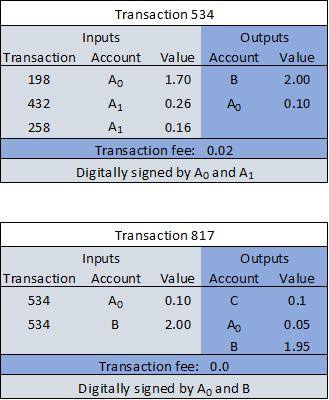
\includegraphics[scale=0.7]{TransactionExample.png}
	\caption{Example of two BTC transactions (adaptation of \cite{DSAwithTime}).}
	\label{fig1}
\end{figure}

Alice sends her new transaction to each of her Bitcoin peers, where it is added to a temporary pool of unverified transactions. Before it is further propagated down the network, Alice's peers verify the new transaction, which includes validation of the UTXOs referenced as inputs and the participating members. After verification, the transaction is added to a pool of valid transactions (\textit{memory pool}) and is sent to the next peers \cite{antonopoulos2017mastering}.

\subsection{Blocks}
For transactions to be confirmed and added to the ledger of valid transactions in the blockchain, they first have to be included in a block and the \textit{proof of work} (Section \ref{pow}) has to be calculated. Potential transactions for the next block are selected from each node's memory pool, whereas transactions with higher fees are prioritized. The main parts of a Bitcoin block are depicted in \autoref{fig2} and consist of a block \textit{header} and \textit{body}. The block header includes the current version of the Bitcoin protocol, a timestamp of the block creation, a hash\footnote{More specifically the root of a merkle tree built from all transaction \cite{okupski2014bitcoin}.} of this block's body and a double-SHA256 hash of the previous block's header. When a new block is created, its previous block field is set to the hash of the most recent block currently on the blockchain. By inserting this hash into the new block, the two blocks are interlinked and the blockchain is extended. This leads to a continuous backwards connection of all blocks up to the \textit{genesis block}. The genesis block is the first block created by Satoshi Nakamoto in 2009 and is statically encoded in each Bitcoin client's software \cite{antonopoulos2017mastering}. Two additional fields, the current mining difficulty and a nonce, are used to calculate the proof of work. The block body contains all transactions added to this block, including a \textit{coinbase transaction} which will be redeemed by the first node successfully calculating this block's proof of work. The coinbase transaction contains the sum of all transaction fees included in the block and the current \textit{block reward}. Giving rewards for mining a block is Bitcoin's way of releasing new BTC to the network and providing an incentive for miners to contribute their resources to the system \cite{okupski2014bitcoin,antonopoulos2017mastering}.
\begin{figure}[ht]
	\centering
  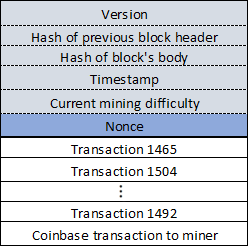
\includegraphics[scale=0.7]{BlockExample.png}
	\caption{Structure of a Bitcoin block \cite{DSAwithTime,okupski2014bitcoin}.}
	\label{fig2}
\end{figure}

\subsection{Proof of Work} \label{pow}
To add a block to the blockchain, a valid proof of work has to be calculated, which is also known as \textit{mining} a block. To mine a block, the node (\textit{miner}) repeatedly calculates the double-SHA256 hash of the block's header, while updating the nonce value. The proof of work is treated as valid once the calculated hash is smaller than a specific target number, which is called the \textit{mining difficulty}. Since SHA256 is considered to be irreversible, brute-forcing the nonce value to generate a new hash each time is the most efficient way of mining a block. The difficutly target is specified in the block header and decreases over time, which consequently increases the difficulty of mining a block. This is done in order to keep the network from mining more than the intended average of six blocks per hour, while hardware and computational power increases. The validity of a block's proof of work can easily be verified by hashing its header once again and testing the result against the target mining difficulty. Since a single node rarely has enough computational power to calculate a valid proof of work in a reasonable time, miners often collude in \textit{mining pools} by sharing any generated block reward based on the amount of hashes calculated by each node \cite{antonopoulos2017mastering,okupski2014bitcoin}.

Since every change in a block's header results in a different hash, calculating the proof of work ensures that once a block has been added to the blockchain the block and its transactions can only be modified by recalculating the proof. In fact, each block that was added after the modified block would have to be recalculated as well, since each block contains the hash of its previous block. By changing the hash of a block, the header of the following block would also have to be changed, thereby invalidating its proof of work \cite{nakamoto2008bitcoin}.

\subsection{Peer-to-peer Network} \label{peer2peer}
After the valid proof of work is computed, the successfully mined block is appended to the local blockchain copy and sent to the miner's peers. Before adding the new block to their own copy of the blockchain and further propagating it in the network, the peers ensure that there exists a hash of any block in their blockchain that corresponds to the hash specified in the new block's header. Blocks without a known parent are called \textit{orphaned blocks}\footnote{In literature orphaned blocks are sometimes used as a term for valid blocks that are no longer part of the main chain after a fork. According to \cite{staleblocks}, we will refer to these blocks as stale blocks instead.} and are temporarily stored, since the missing parent block might be transmitted in the future. If the new block does reference an existing block in the blockchain, contains only valid transactions and satisfies the current mining difficulty with its proof of work, the block is appended to the correct parent in the local blockchain and sent to the next peers. 

Because Bitcoin operates on a peer-to-peer basis, latencies in the network are unavoidable. According to \cite{infoprop}, the mean time until a
node receives a new block is 12.6 seconds, while approximately 5\% of nodes still have not received the block after 40 seconds. Since a new Bitcoin block is created \textit{on average} every 10 minutes, it is possible that two miners find solutions to two different blocks at roughly the same time, thereby creating a \textit{fork} or \textit{branch} of the blockchain (\autoref{blockchainfork}). This results in a situation in which the local blockchain copies of some peers are no longer synchronized. To resolve this conflict and to regain consensus between nodes, a simple rule is employed. According to the bitcoin protocol, nodes are always mining on the blockchain containing the most proof of work which approximatley corresponds to the fork with the highest number of blocks. If two forks containing the same amount of blocks are available, miners are encouraged to work on the fork they received first. This ensures that even if there are two versions of the blockchain with the same length, nodes will keep mining on any of the two forks until a new block is found. By appending the new block to one of the forks, the contained proof of work increases and miners working on the other fork will switch to the longer chain, thereby resolving the race. Subsequently, the blocks of the losing fork are invalidated and become what is known as \textit{stale} blocks \cite{okupski2014bitcoin}. Transactions are only considered to be confirmed if they are part of the longest, valid chain. The transactions contained in stale blocks that are not yet part of the main chain are consequently mined into new blocks on the longest chain, as long as the specified inputs of the transaction are still valid. Stale branches of the blockchain are still stored as a part of all local blockchain copies. If enough blocks extending a stale branch are received for it to become the longest chain, the stale blocks will be considered valid again and the now longest branch is declared as the main blockchain.
\begin{figure}[ht]
	\centering
  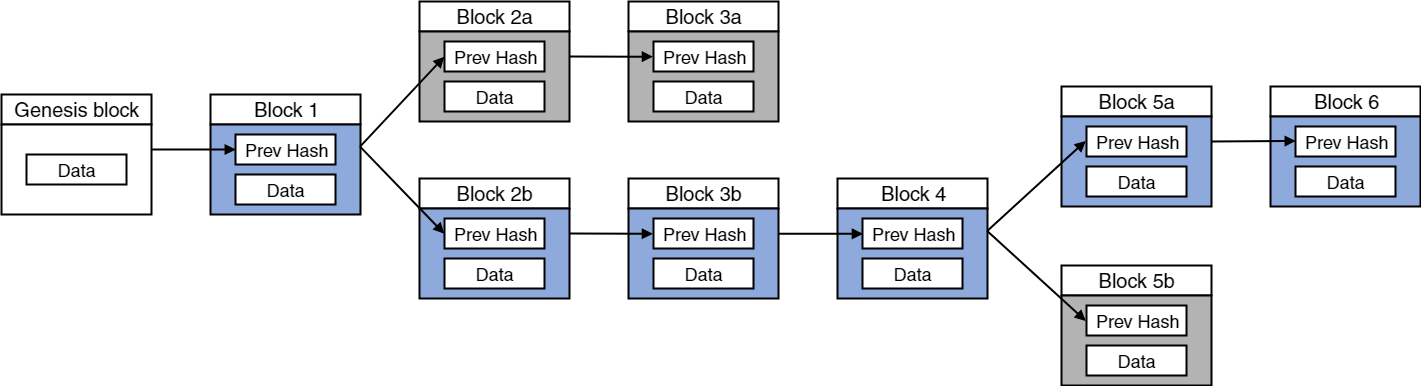
\includegraphics[width=\textwidth]{BlockchainFork.png}
	\caption{Blockchain with two stale branches (gray) forking from the valid chain (blue). }
	\label{blockchainfork}
\end{figure}

To avoid problems with invalidated blocks and transactions due to these kinds of races and attacks similar to the one presented in Section \ref{pow}, Bitcoin introduced the concept of \textit{confirmations}. If Alice's transaction is validated and successfully mined into a block on the main blockchain, it receives \textit{one} confirmation. For each additional block mined onto the chain, after the block containing Alice's transaction, it receives another confirmation. Consequently, the number of confirmations corresponds to the number of blocks that would have to turn stale, or have to be recalculated, in order to invalidate Alice's transaction. Over the history of Bitcoin, the number of six confirmations has been widely accepted as a common standard. However, since waiting for six confirmations means waiting approximately one hour for the transaction to be valid, a lot of services operate on only a few or even no confirmations, which can lead to several problems further described by \cite{premining1}. In comparison, coinbase transactions to reward the miner of a new block are considered to be valid only after they have been confirmed by a total of 100 mined blocks \cite{antonopoulos2017mastering}.

\section{Double-Spend Attacks} \label{dsa}
\begin{sloppypar} In \cite{nakamoto2008bitcoin}, Nakamoto claims to have solved the double-spending problem with his proposal of the Bitcoin protocol. Nevertheless, attacks on Nakamoto's blockchain architecture to generate double-spending transactions are still possible and can be described as a series of events: \end{sloppypar}
\begin{enumerate}
\item An attacker \textit{A} would like to receive a service or product from a target merchant \textit{M}.
\item \textit{A} generates two transactions:
\begin{itemize}
\item \textbf{T\textsubscript{M}}, to pay the merchant.
\item \textbf{T\textsubscript{A}}, to send the money back to \textit{A}. Created by specifying \textit{A} as output while using the same inputs of \textbf{T\textsubscript{M}}.
\end{itemize}
\item \textit{A} broadcasts \textbf{T\textsubscript{M}} and starts mining on a secret branch extending the most recent block. \textit{A} includes \textbf{T\textsubscript{A}} into the first block of the new branch.
\item Once \textbf{T\textsubscript{M}} is confirmed by the remaining network, \textit{M} delivers the product or service to \textit{A}.
\item If necessary, \textit{A} keeps mining on the secret branch containing \textbf{T\textsubscript{A}} until it is longer than the honest branch containing \textbf{T\textsubscript{M}}.
\item \textit{A} releases her now longer branch, thereby invalidating each block of the honest branch, including the block containing \textbf{T\textsubscript{M}}.
\item All nodes start mining on the longer branch. Since \textbf{T\textsubscript{A}} is now part of the valid blockchain, the inputs for \textbf{T\textsubscript{M}} are already used. As a result of this, \textbf{T\textsubscript{M}} cannot be re-added to the new longest chain because the specified inputs are invalid. Consequently, \textit{A} gets to keep \textit{M}'s payment as well as the delivered product.
\end{enumerate}
For this attack to succeed, \textit{A} is required to mine blocks onto the secret blockchain branch faster than the remaining network confirming the transaction to the merchant. According to \cite{nakamoto2008bitcoin}, consistently winning this race requires the majority of hashing power in the network. Nevertheless, this attack is always possible even with less hashing power at the cost of an increasing amount of failed attempts \cite{HBDSA,DSAwithTime}.


%------- chapter 3 -------

\chapter{Related Work} \label{relatedwork}
To identify parameters affecting the resistance of blockchain architectures against double-spend attacks and to gain an understanding of existing literature regarding general attacks on blockchains and their modeling, we will review a selection of related work. The following provides an overview of the reviewed literature and summarizes the authors' conclusions that are relevant to our investigations.
\section{Hashrate-based Models for Double-Spend Attacks}
\begin{sloppypar}
Potential attacks on blockchains, especially the Bitcoin protocol, have been conceptualized since the release of Nakamoto's original Bitcoin paper \cite{nakamoto2008bitcoin}. In chapter 11 of his proposal, Nakamoto formulates the first mathematical model to calculate the theoretical probability of successful double-spend attacks on his protocol. This model has since been improved and adapted several times, while similar, independent models have been formulated as well \cite{HBDSA,DSAwithTime,NakamotoDSACorrection,NakamotoExplMCSim}. Similar to \cite{DSAwithTime}, we will call the collection of these approaches \textit{hashrate-based} attack models. The central premise of a hashrate-based model is splitting the total computing power available to the network (hashrate \textit{H}) into two parts. To achieve this, \cite{HBDSA} defines \textit{pH} as the hashrate controlled by honest nodes adhering to the protocol, while \textit{qH} is used by malicious nodes trying to attack the blockchain. Since also\end{sloppypar}
\begin{equation}
p + q = 1,
\end{equation}
it can easily be seen that \textit{p} and \textit{q} are precisely the probabilities of the next block being mined by either the honest or the attacking part of the network. Using an adaptation of the Gambler's Ruin problem \cite{gamblersruin}, Nakamoto and \cite{HBDSA} are now calculating the probability \textit{Q\textsubscript{z}} of an attacker successfully catching up with their fork of the blockchain, asuming they are at a total deficit of \textit{z} blocks compared to the honest nodes. The success of a potential double-spend attack against a merchant waiting for \textit{n} confirmations can now be formulated as the probability of \textit{Q\textsubscript{z}}, after \textit{n} blocks have been mined by the honest network. While \cite{nakamoto2008bitcoin} is using a poisson distribution in his formula, \cite{HBDSA} is achieving similar results with a negative binomial distribution. Combined with \cite{NakamotoDSACorrection}, the author of \cite{HBDSA} is also pointing out and correcting an of-by-one error introduced by Nakamoto, who is only calculating the probability of an attacker \textit{catching up} with his fraudulent blockchain fork, while for the double spend attack to be successful, the length of the honest chain has to be \textit{surpassed}. \cite{DSAwithTime} presents two similar approaches but considers partial advancement towards block creation as well. The author's first model extends the hashrate-based model formulated by \cite{HBDSA} and includes an additional parameter, indicating the time an attacker has already spent mining on blocks. The second model is fundamentally based on the time differences at which honest and attacking nodes have mined their last block, but is also relying on hashrates as a measure of computational power.
It is interesting to note that all of the previously mentioned models produce similar results despite the differences in their calculations. Therefore it is less surprising that the authors seem to agree on their general conclusions as well. Those can be summarized as follows:
\begin{itemize}
\item If an attacker controls the majority of computational power in the network, double-spend attacks will always succeed.
\item Probabilities for successful double-spend attacks decrease exponentially with an increasing number of confirmations.
\item Probabilities for successful double-spend attacks increase exponentially with an increasing amount of hashing power controlled by the attacker.
\item Although double-spend attacks at the standard of six confirmations are considered to be unlikely, there is nothing special about the number six.
\item Double-spend attacks are always possible regardless of the number of confirmations and amount of computational power controlled by the attacker.
\end{itemize}
\section{Simulations}
An important remark can be seen in the fact that none of the before mentioned hashrate-based models have been confirmed or supported by experimental data or tests in an exhaustive and realistic way. Instead, the validity of these models relies mostly on mathematical proofs and expertise, or the comparison with other, similar models. Nevertheless, one exception can be made with \cite{NakamotoExplMCSim}. After presenting a detailed explanation of Nakamoto's model for double-spend attacks, the author validates the mathematical approach by performing a Monte Carlo simulation \cite{montecarlo} with different sets of input. In the light of this, the author identifies an error of the model, which is linked to its use of the poisson distribution. In spite of this success, the Monte Carlo simulation is missing parameters of a real blockchain protocol and ``does not actually mine coin, it simply flips some coins to see whether each miner wins a block as simulated'' \cite{NakamotoExplMCSim}. A more realistic simulation of a different attack on Bitcoin blockchains, the \textit{selfish-mine} attack, is presented by \cite{mwalemodel} and \cite{selfishmine2}. In these two models of the Bitcoin protocol, random (\textit{x}, \textit{y})-coordinates of a two dimensional plane are assigned to each node in order to create a simple network topology. By simulating the latency between two nodes as proportional to their euclidean distance in the plane, both authors successfully model block propagation times of a real network. During the simulation, new blocks are again generated as instances of a poisson process with an average rate of ten minutes. 
\section{Other Attacks} \label{otherattacks}
Next to double-spend attacks a wide variety of different attacks against blockchains and the Bitcoin protocol have been conceptualized. The already mentioned \textit{selfish-mine attack} or \textit{block-discarding attack}, focuses on invalidating the honest miners' work by selectively publishing premined blocks to the network \cite{mwalemodel,selfishmine1,selfishmine2,lessThanHalfDraft}. According to \cite{lessThanHalfDraft} and \cite{selfishmine1} this attack can succeed with only a fraction of 25\% total hashing power controlled by the attacker. The \textit{whale attack} presented by \cite{whaleattack} aims to increase an attacker's chances of successful double-spends by publishing transactions with large mining fees to incentivize honest miners to build on a fraudulent blockchain fork. \cite{premining1} and \cite{premining2} further capitalize on the \textit{premining} strategy of secretly mining blocks ahead of the honest blockchain, while also including a reversed transaction to the target. Once the attacker has gained a comfortable lead, the original transaction to the target merchant is released. Now the lead of the attackers' fork only has to be maintained until the transaction has been confirmed, in order to perform a double-spend. The authors demonstrate how this attack can be used to increase the probability of double-spend attacks, when timing of the transaction used as bait is not important.
\section{Contribution} \label{contribution}
It can clearly be observed that despite the considerable amount of work being done towards the formalization of theoretical attack models against blockchains and especially double-spends attacks, barely anything has been validated by empirical evidence or data. Instead, correctness of the proposed models is achieved by mathematical proofs, while arguably important factors of blockchain dynamics are disregarded or hidden behind intangible parameters like the ``hashrate''. In this thesis we will therefore counter this trend and design a \textit{Java} framework to model simulations of blockchain architectures. This framework will subsequently be used to implement an exemplary simulator for double-spend attacks. The goal is to increase the understanding of factors affecting the resistance of blockchain architectures against double-spend attacks and to improve an architect's predictions based on results generated by the model. This will be achieved by conducting experiments based on real world inspired parameters of a blockchain protocol using our simulator. The simulator therefore allows configuration of different parameters, which were identified by reviewing literature concerning blockchain architectures (see for example \cite{nakamoto2008bitcoin,antonopoulos2017mastering,HBDSA,infoprop}) and are assumed to influence the amount of successful double-spends during operation. These parameters include:
\begin{itemize}
\item The number of attacking and trusted nodes
\item The difficulty of mining a new block
\item The number of confirmations required by the target
\item Topology and density of the attacking and defending network
\item Latency in the attacking and defending network
\item Latency of the connection between attacking and defending network
\end{itemize}
Using these parameters and the simulator framework, we will then propose our own empirical model for double-spend attacks, based on data generated by several experiments and tests.
%------- chapter 4 -------

\chapter{The Blockchain Simulator} \label{simulator}
The blockchain simulator consists of a framework enabling the simulation of general blockchain architectures (Section \ref{simframework}) and an exemplary application of the framework resulting in the double-spend simulator (Section \ref{dssim}). The latter represents an implementation of a blockchain architecture targeted by continuous double-spend attempts, which are initiated by an attacking network. The simulator allows individual configuration of the parameters identified through literature in Section \ref{contribution} in order to model various architectural scenarios. To analyze the effects of these parameters, the double-spend simulator measures the percentage of successful double-spend attacks ($PDS$) after a series of attempts, as well as the percentage of stale blocks (Section \ref{peer2peer}) generated by the attacking network ($PSB_A$) and the trusted network ($PSB_T$). The following provides an overview of the simulator's architecture and components. The general usage of the simulator and its modeling of the parameters are described in Section \ref{usage}.
\section{Simulation Framework} \label{simframework}
To simplify future implementation and simulation of other attacks on block\-chains, the core part of our simulator represents an extensible, abstracted framework for general blockchain architectures. By subclassing the existing elements of the framework, the simulator's functionality can be extended and customized in order to model specific blockchain dynamics. Compared to the example blockchain protocol presented in Section \ref{bitcoin}, a few adaptations have been made:
\begin{itemize}
\item Every node of the network is a miner.
\item Each miner is represented by a single program thread.
\item Instead of hashing a block and updating nonce values, mining a block consists of repeatedly generating random numbers until a number lower than the target difficulty is found.
\item The framework does not include generation and transmission of transactions, since the data contained inside the blocks does not affect the behavior of blockchain architectures.
\item Instead of sending single blocks, miners propagate whole copies of their local blockchains along the network.
\item Nodes start mining on a received blockchain if it is longer than the blockchain currently being mined on.
\item Latency time between two peers is constant.
\end{itemize}
\subsection{Classes}
\autoref{umlframework} represents the UML class diagram describing the simulation framework's architecture. The network class consists of all ($n$) nodes modeled in the simulation. Each node maintains references to $n-1$ peers and their corresponding latency times. The node mines on its local blockchain copy which is shared with all peers once a new block is found. Names written in \textit{italics} represent the framework's abstract classes and functions.
\begin{figure}[ht]
	\centering
  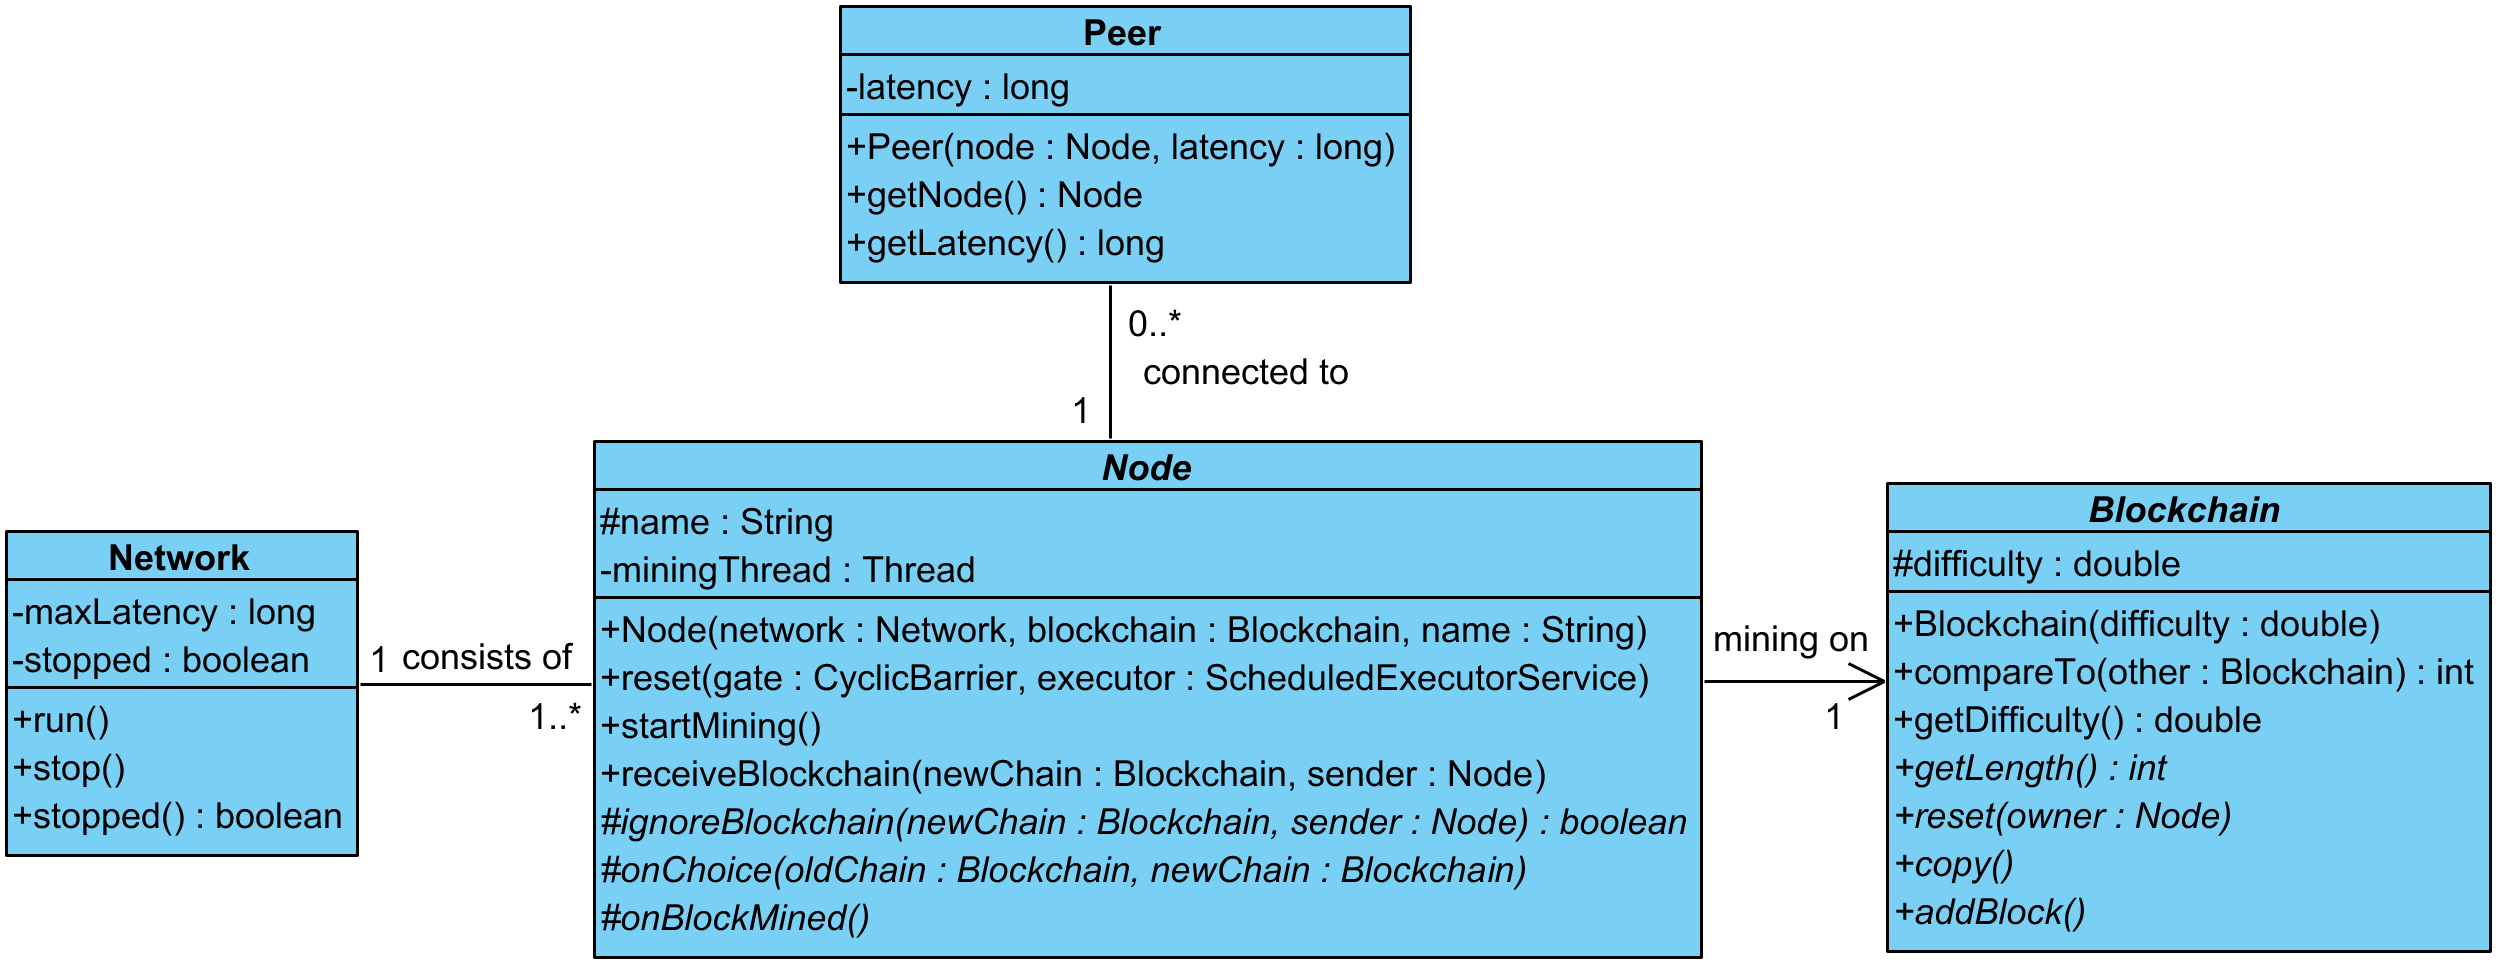
\includegraphics[width=\textwidth]{Framework.png}
	\caption{UML class diagram of the blockchain simulation framework.}
	\label{umlframework}
\end{figure}

\subsubsection{Node}
The node represents a basic implementation of an honest miner adhering to our blockchain protocol. Each node contains a reference to every other node in the network using the peer class. Once a new block is mined, it is added to the local blockchain and, after the corresponding latency times, a copy of the blockchain is sent to all peers. The node will only start mining on a newly received blockchain if it is longer than the local blockchain copy. To simplify execution of multiple simulation runs, each node can be reset to its initial state. To allow simulation of nodes diverging from the standard protocol, the class contains three abstract methods which can be implemented to alter the behavior of the node. 

\subsubsection{Peer}
To represent the connection to a node in the network, the peer is implemented as a simple data class without further functionality, containing the latency time in milliseconds needed to reach the referenced node.

\subsubsection{Blockchain}
In order to allow concrete implementations of different blockchain models, the blockchain class only provides the abstracted interface required by nodes. An implementation of the blockchain class therefore contains routines for adding a block and returning the length of the blockchain. Since nodes propagate whole copies of the blockchain instead of single blocks, a method of copying the blockchain has to be implemented as well.

\subsubsection{Network}
The network acts as a central controller of the blockchain framework. It maintains references to all nodes in the network and provides simple routines for starting and stopping the mining processes of all nodes in a synchronized manner. Once the network is started, the calling thread of \textit{run()} is blocked until the execution of all nodes is completed. The nodes terminate their mining threads after the network is stopped, which is ideally done as a consequence of some end condition reached by the simulation.


\subsection{Creating the Peer-to-peer Network} \label{peerstratsection}
Apart from simulating blockchains and miners, the simulator framework offers additional functionality to model different forms of peer-to-peer networks. The general task is to create a connected graph of all nodes, whereas the graph's edges represent direct peer connections between nodes and the edge weights correspond to the latency times applied to each connection. Using the strategy pattern\cite{strategy}, the simulator framework provides implementations of five different ways of modeling the network (\autoref{peerstrategy}), while additional strategies can easily be added in the future. The different peer strategies are used by instantiating the specific strategy and calling the \textit{connectPeers()} method with a list of all nodes in the network. The strategy will then populate the peer lists of each node accordingly. In the following, an overview of all available strategies will be provided.
\begin{figure}[ht]
	\centering
  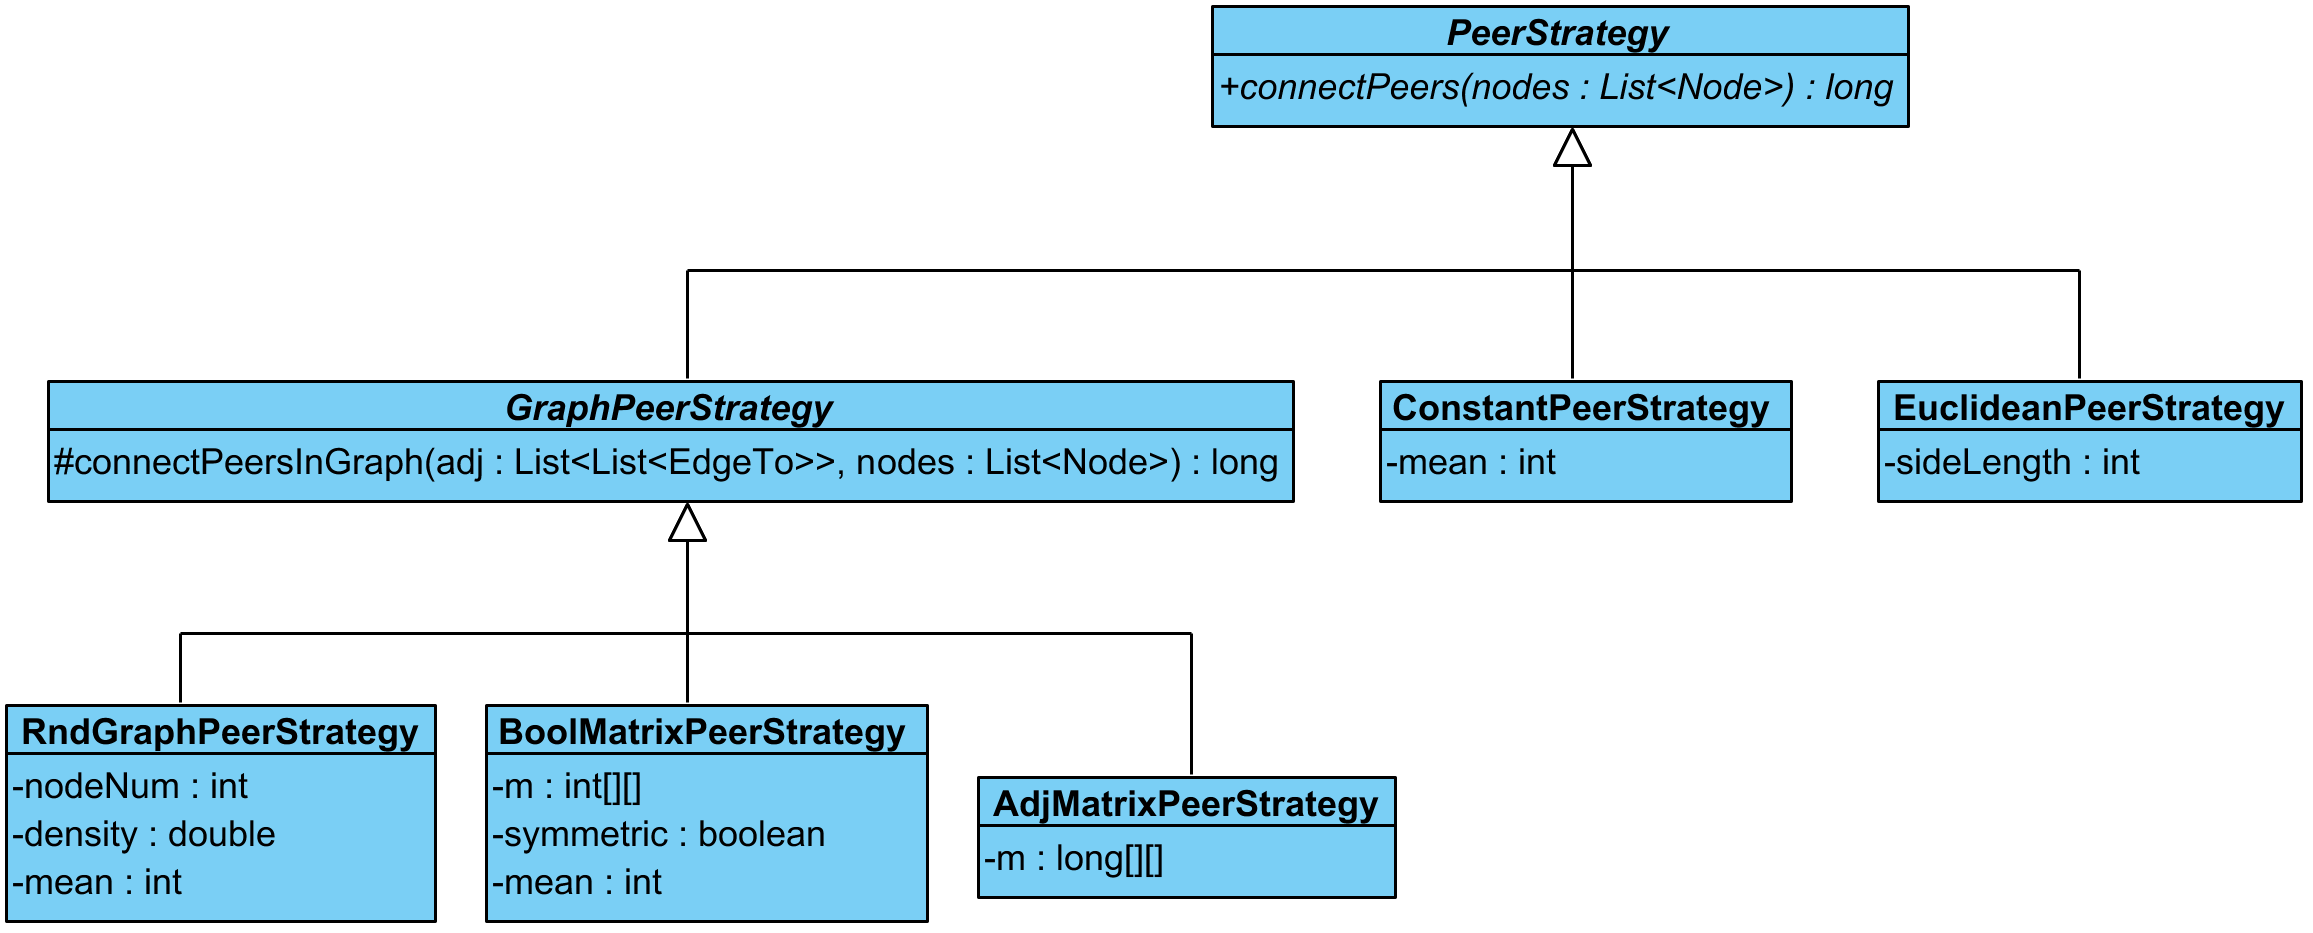
\includegraphics[width=\textwidth]{PeerStrategy.png}
	\caption{UML class diagram of the different strategies available to connect nodes in the peer-to-peer network.}
	\label{peerstrategy}
\end{figure}
\subsubsection{ConstantPeerStrategy}
All nodes in the network are connected by latencies $l$, sampled from a random variable $L$ which is following a normal distribution with constant mean $m$. The standard deviation is calculated using a constant deviation factor $c$ and the mean (\autoref{distribution}). Unless otherwise specified, $c$ equals $0.1$.
\begin{equation}\label{distribution} 
l\in L\sim cm\mathcal{N}(0,1)+m = \mathcal{N}(m,c^{2}m^{2})
\end{equation}
\subsubsection{EuclideanPeerStrategy}
Similar to the models presented by \cite{mwalemodel} and \cite{selfishmine2}, all Nodes are assigned random coordinates $(x,y)$ in a two dimensional, quadratic plane. The latency between two Nodes $p$ and $q$ is sampled from the normal distribution defined in \autoref{distribution}, whose mean $m$ is equal to the nodes' euclidean distance (\autoref{euclid}).
\begin{equation}\label{euclid}
m = \sqrt{(p_{x}-q_{x})^{2}+(p_{y}-q_{y})^{2}}
\end{equation}
By setting the strategy's \textit{side length} parameter, the area of the square can be defined. Creating a bigger plane consequently leads to overall higher latencies in the network.
\subsubsection{AdjMatrixPeerStrategy}
This strategy creates a graph of nodes according to an adjacency matrix which is provided as an input when instantiating the strategy. Latencies between two nodes are represented by the matrix entries, whose indices refer to the corresponding nodes in the provided list. Negative entries indicate that there is no connection between two nodes, whereas a value of zero leads to a connection without any latency. Choosing the entry values allows simulation of typical network topologies like stars and rings. After creating the graph, Dijkstra's shortest path algorithm \cite{dijkstra} is used to solve the all pairs shortest path (APSP) problem. With the resulting distance matrix, all peers of each node can be initialized.
\subsubsection{BoolMatrixPeerStrategy}
Similar to the previous strategy, a graph is created as specified by the given adjacency matrix. This time, positive entries of the matrix only indicate existence of a connection between two nodes, whereas negative and zero values lead to no connection in the graph. The latencies are instead sampled from a normal distribution with constant mean as defined by formula \ref{distribution}.
\subsubsection{RndGraphPeerStrategy} \label{rndgraphstrategy}
This strategy generates a pseudo-random graph with a given number of nodes and edges. To reduce the scale of a parameter defining the number of edges, a graph density parameter is used to calculate the number of edges. The graph or network density describes the ratio of existing edges to the maximum possible number of edges and is therefore represented by values between zero and one for every graph \cite{density}. This ratio $d$ can be calculated for undirected graphs as shown in \autoref{dense}, where $n$ and $e$ denote the number of nodes and edges, respectively. Since the generated graph is required to be connected, the number of edges $e$ used by the strategy is calculated from $d$ and $n$ as shown in equation \ref{dens}. 
\begin{equation}\label{dense}
d = \frac{2e}{n\left( n-1\right) }
\end{equation}
\begin{equation}\label{dens}
e = max \left( d\frac{n\left( n-1\right) }{2}, n-1 \right),\quad d\in [0,1]
\end{equation}
Edge weights of the graph corresponding to the latency between two nodes are sampled according to formula \ref{distribution}. The distances between all nodes required to initialize each node's peers are again calculated by Dijkstra's APSP algorithm. 

\section{Double-Spend Simulation} \label{dssim}
In order to simulate double-spend attacks, we split the miners modeled by the blockchain framework into two parts and create two subclasses of the framework's node implementation. The newly created, trusted nodes adhere to our simplified blockchain protocol and keep mining on the longest branch they are currently aware of. The dishonest nodes, trying to generate a double-spending transaction, are mining blocks to extend their secret branch. Both groups of nodes are combined into an attacking and trusted network by using two instances of the peer strategies presented in Section \ref{peerstratsection}. Unless otherwise specified, the double-spend simulator uses two \textit{RndGraphPeerStrategies} and recreates the resulting graphs randomly before every new simulation run. Initially, consent of all nodes is on a blockchain of size 0, containing the most recent block before \textbf{T\textsubscript{M}} and \textbf{T\textsubscript{A}} are published. \textbf{T\textsubscript{M}} and \textbf{T\textsubscript{A}} correspond again to the transactions created by the attacker as defined in Section \ref{dsa}. While \textbf{T\textsubscript{M}} represents the legitimate payment to the merchant, which is published to the honest network, \textbf{T\textsubscript{A}} is used to revert the payment and is incorporated into the secret branch mined by the attacker. Since all blocks added to the trusted blockchain before \textbf{T\textsubscript{M}} is included could simply be added to the attackers' branch without any computation, it is assumed that both transactions are mined into the first block of their corresponding networks. After \textbf{T\textsubscript{M}} is confirmed with the simulated number of confirmations, the merchant's product is assumed to be sent. The attackers then start publishing their branch including \textbf{T\textsubscript{A}}, to convince the trusted network of their alternate transaction history not containing \textbf{T\textsubscript{M}}. The double-spend is considered to be successful once all trusted nodes are mining on the blockchain containing \textbf{T\textsubscript{A}}.
\subsection{Classes}
\autoref{simulation} represents the UML class diagram of the double-spend simulator's architecture. The \textit{DSSimulation} class uses two \textit{PeerStrategy} instances to connect the nodes in the attacking and trusted networks, as well as one \textit{ConnectionStrategy} instance to connect both networks with each other. Grey classes represent components of the simulator framework, which are further described in figures \ref{umlframework} and \ref{peerstrategy}. By subclassing the \textit{Node} and \textit{Blockchain} classes, the framework's functionality is extended in order to model the behavior of trusted and attacking nodes, as well as to differentiate between blockchains containing \textbf{T\textsubscript{M}} or \textbf{T\textsubscript{A}}. All events of nodes finding new blocks or accepting fraudulent blockchains are reported to the \textit{DSManager} instance, which determines the end of a double-spend attempt and initiates the next simulation run by reporting the results to the \textit{DSSimulation} instance.
\begin{figure}
	\centering
  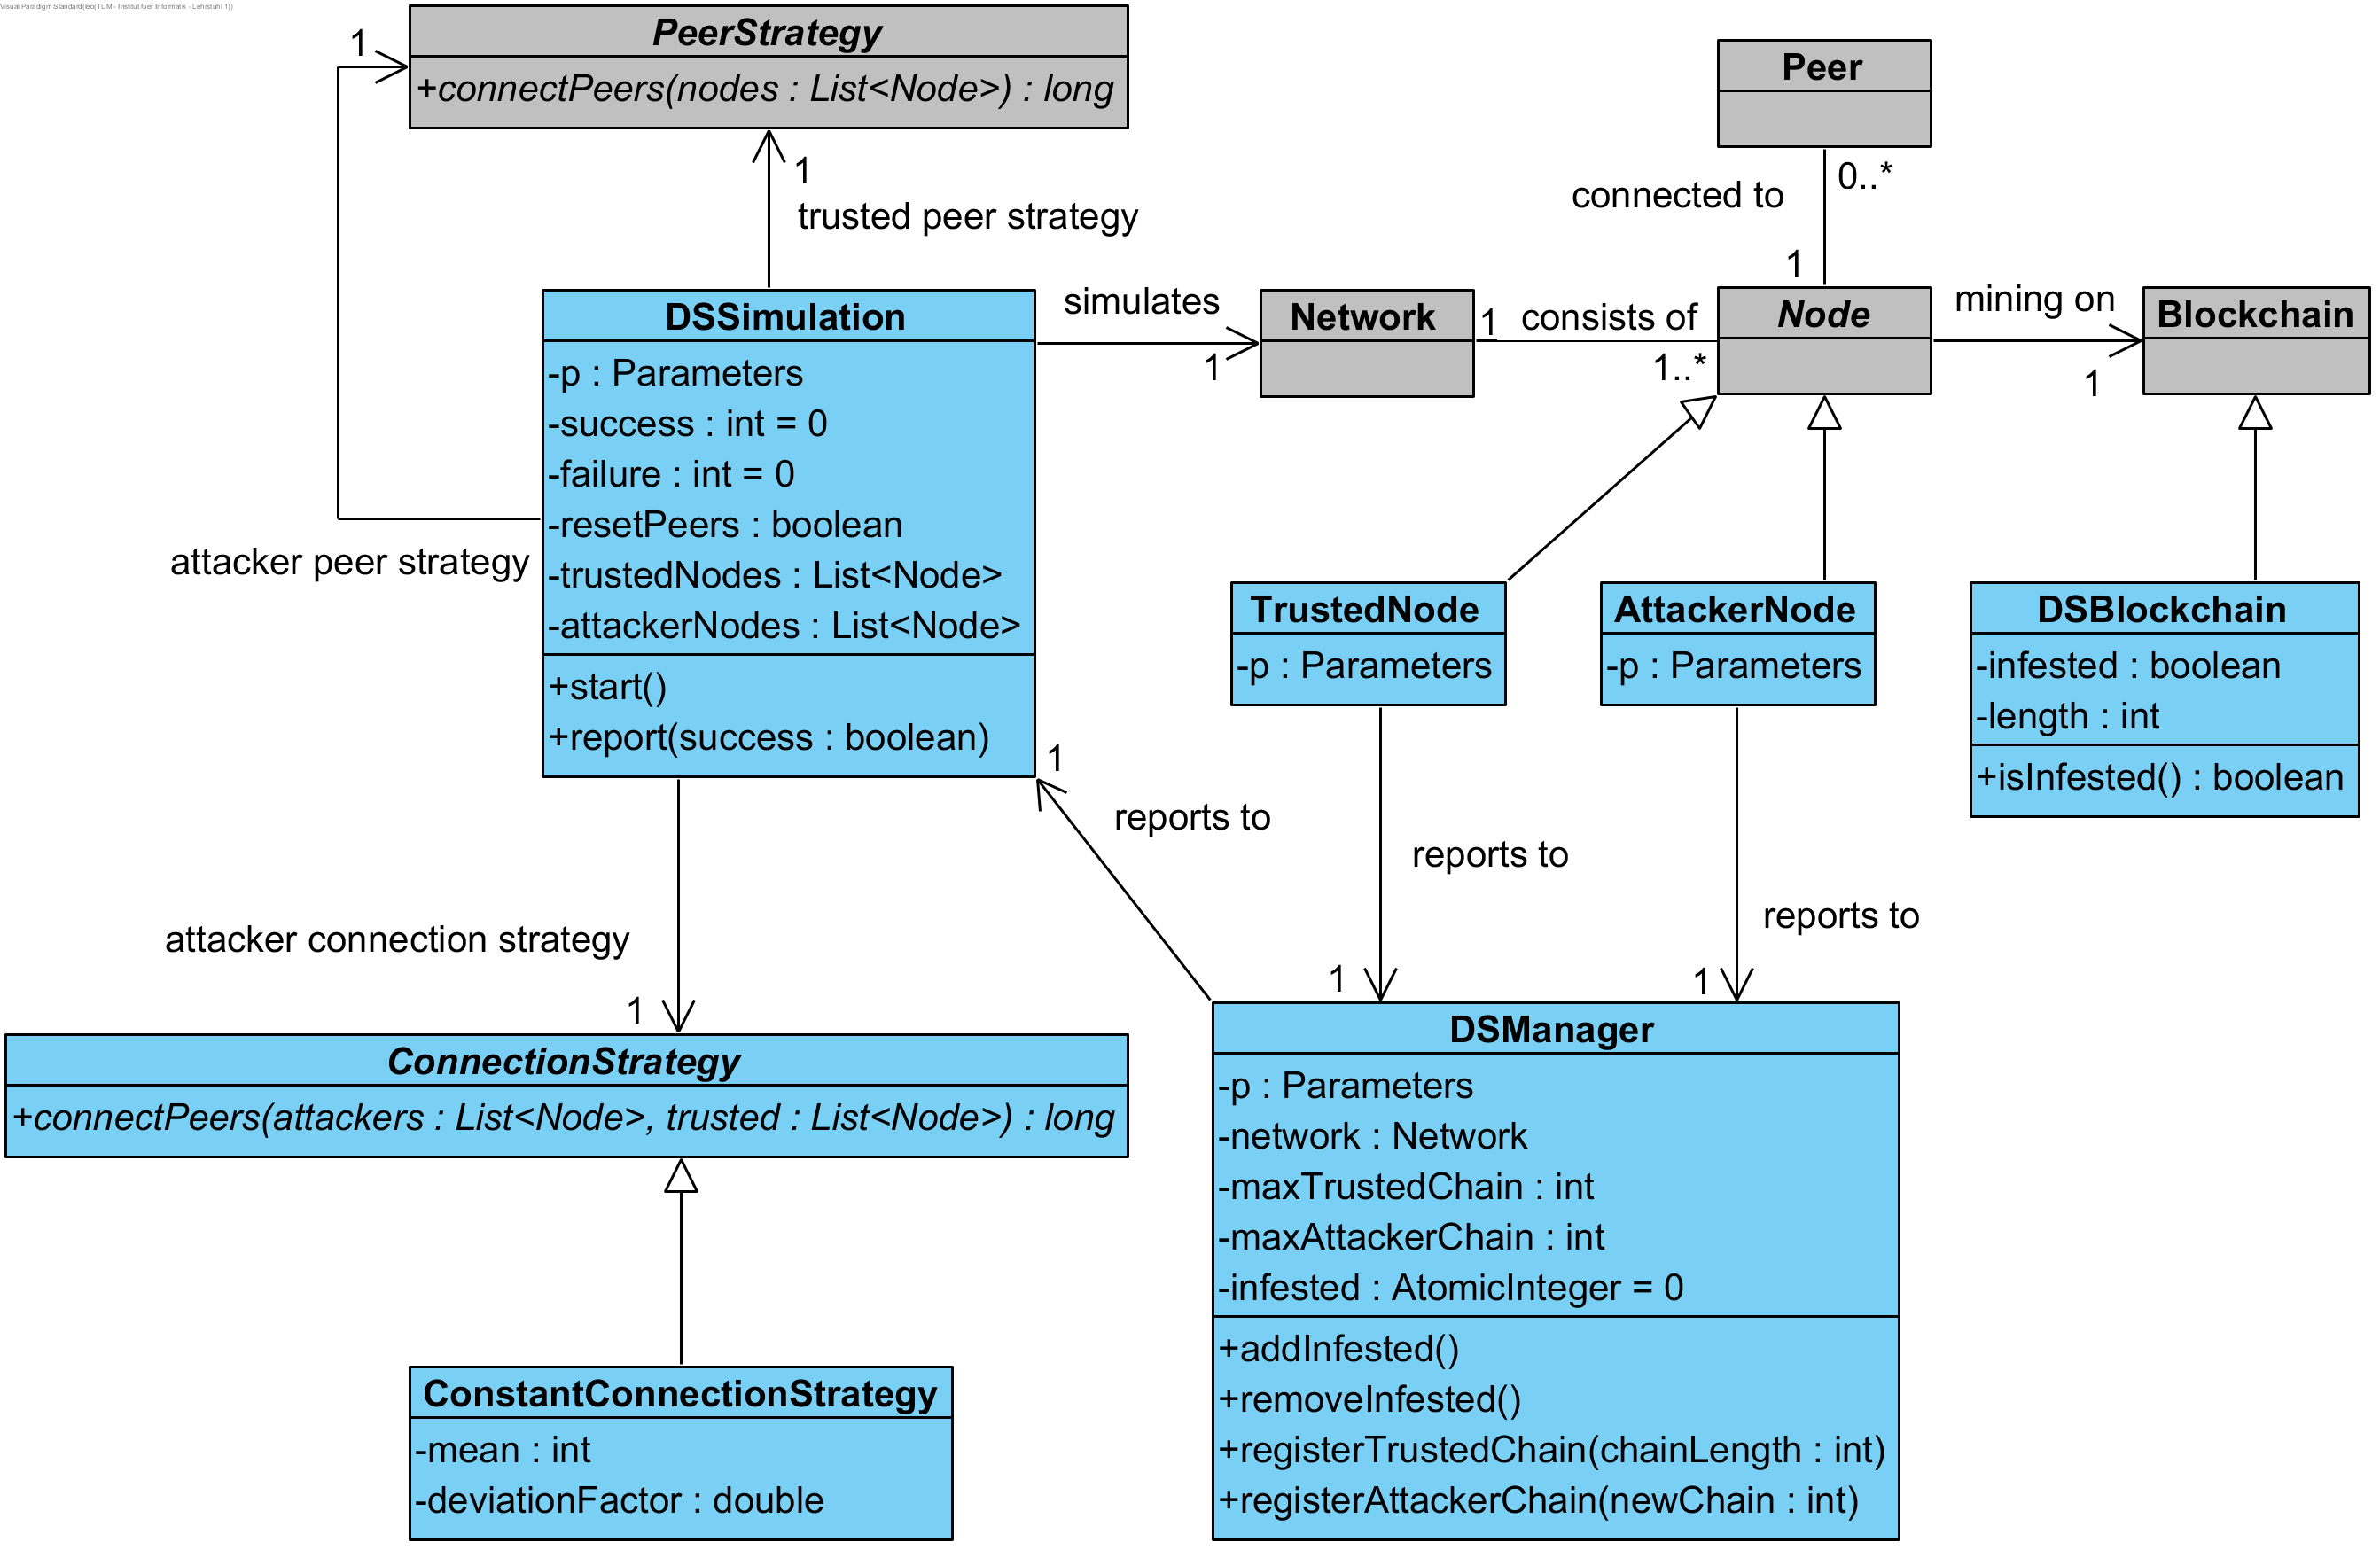
\includegraphics[width=\textwidth]{Simulation.png}
	\caption{UML class diagram of the double-spend simulation.}
	\label{simulation}
\end{figure}
\subsubsection{DSSimulation}
The \textit{DSSimulation} initially creates all other instances of this simulation, including the network and its nodes. The class represents the central controller of the simulation, keeping track of successful and failed double-spend attempts and the total number of runs. Once a run is completed, the current attempt is stopped by communicating with the network and the next run is initiated. Parameters and the peer-to-peer graph can be recreated every run to allow randomization of different simulation aspects. The simulation is generating measures regarding the percentage of successful double-spends compared to the total number of attempts, as well as the percentage of stale blocks created by both networks.
\subsubsection{DSBlockchain}
The blockchain used to simulate double-spend attacks. Instead of modeling entire blocks, the \textit{DSBlockchain} only consists of its length, which is incremented every time a new block is added. Since double-spend attacks resolve around winning the race between the attackers' and the honest nodes' blockchains, only the number of blocks in the chain is relevant and modeled by our simulation. It is important to note that by representing the blockchain only by its length, we are not explicitly distinguishing between stale and valid blocks. However, the effects of stale blocks and branches still exist in the network. 

Imagine the current consensus in the network to be a blockchain of length 3. If now two nodes mine a new block at approximately the same time, both nodes send blockchains of length 4 to every peer. In the original protocol, this would result in two different blockchains of length 4 being spread across the network, but using our model they are indistinguishable. Nevertheless, the nodes of our network simulation still experience one wasted, stale block, as they mined a total of two blocks, but were only able to increase the length of the consented blockchain by one.

To differentiate between blockchains containing the honest payment to the merchant (\textbf{T\textsubscript{M}}) and fraudulent blockchains replacing the payment with a self receiving transaction (\textbf{T\textsubscript{A}}), the DSBlockchain contains a boolean flag indicating whether it is malicious or not.
\subsubsection{DSManager} \label{manager}
A central manager class collecting data sent from every node. By keeping track of the longest attacker and honest blockchains and the amount of nodes mining on a fraudulent chain, the manager determines whether a double-spend attack is successful or if it should be aborted. The attempt of creating a double-spend is considered successful once all nodes are mining on a fraudulent blockchain, after \textbf{T\textsubscript{M}} has been confirmed by each honest node. This corresponds to the network's consent to be on the double-spending transaction \textbf{T\textsubscript{A}}, after the product bought with \textbf{T\textsubscript{M}} has already been shipped (Section \ref{dsa}). 

Since the simulation is potentially running endlessly if the attacking network never succeeds in overtaking the honest network's blockchain, the manager considers two parameters in order to decide if the current attempt should be aborted. Firstly, once a maximum lead of the honest network over the attacking network's blockchain is achieved, the success of a double-spend is deemed to be too unlikely and the current run is aborted in failure. Secondly, to avoid the possibility of the honest network maintaining a steady lead without triggering the first parameter, the simulation is restricted by a maximum length of the blockchains. Once this length is reached by any blockchain the current run fails as well. The second parameter is especially important if both networks contain a similar amount of nodes. The nature of these two parameters is further described in Section \ref{faulttolerance}.
\subsubsection{TrustedNode}
This is the implementation of a honest node in the network, working on adding blocks to the longest chain they are currently aware of. The node originally starts working on confirming \textbf{T\textsubscript{M}} with a, by the simulation specified, number of confirmations. After the transaction is confirmed and the product of Section \ref{dsa} has been sent, the node keeps mining on the longest chain. Consequently, it might start mining on the fraudulent blockchain sent by the attacker, as long as it contains more blocks than the original chain. At this point the trusted node is convinced that \textbf{T\textsubscript{A}} is represented in the correct version of the transaction history. However, if the trusted node subsequently receives a longer blockchain containing \textbf{T\textsubscript{M}}, it will switch back to mining on a honest chain. These infection like alternations are reported to the manager class until all trusted nodes have been convinced by the attackers, or the attempt is aborted.
\subsubsection{AttackerNode}
Contrary to the trusted nodes, the attacking nodes ignore all blockchains not containing the fraudulent transaction \textbf{T\textsubscript{A}} and work exclusively on adding blocks to their private fork. Once \textbf{T\textsubscript{M}} has been confirmed by the trusted network, the attackers start publishing their fraudulent blockchains to convince the network of \textbf{T\textsubscript{A}}.
\subsubsection{ConnectionStrategy} \label{connstrat}
Similar to the framework's \textit{PeerStrategy}, the \textit{ConnectionStrategy} adds edges to the network's graph by populating the lists of peers maintained by each node. Instead of creating edges among nodes of a single network, this strategy allows the connection of sets of nodes with each other. Since the network of attacking nodes needs to be able to send its fraudulent blockchains to the honest nodes, this functionality is used to create a connection between both networks. The \textit{ConnectionStrategy} thereby represents how well the attacking nodes are able to publish their blockchains depending on the connection's latency. The only strategy currently implemented connects all attacking nodes with all honest nodes by sampling latency times from the normal distribution defined in formula \ref{distribution}. \autoref{network} depicts the relationship between peer and connection strategies in their corresponding network.
\begin{figure}[ht]
	\centering
  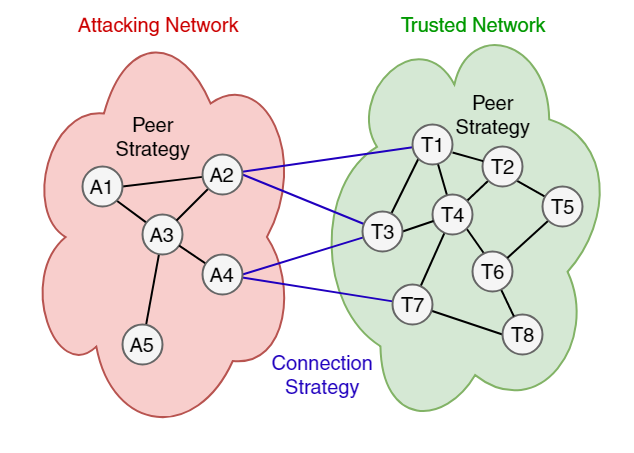
\includegraphics[width=\textwidth]{Network.png}
	\caption{Exemplary simulation network of five attacking and eight trusted nodes.}
	\label{network}
\end{figure}

\subsection{Activity Diagram}
To increase the understanding of the simulator's operation and the interaction of its components, \autoref{activity1} provides an overview of all actions completed by each simulator entity as an UML activity diagram. Note that the \textit{Node} swim lane corresponds to a single trusted or attacking node of the simulation. After starting a new simulation run, all nodes begin mining for new blocks, while simultaneously receiving blockchains sent by their peers. New blocks and the amount of nodes convinced by the double-spending transaction are reported to the \textit{DSManager} which determines the success of the current double-spend attempt.
\begin{figure}[ht]
	\centering
  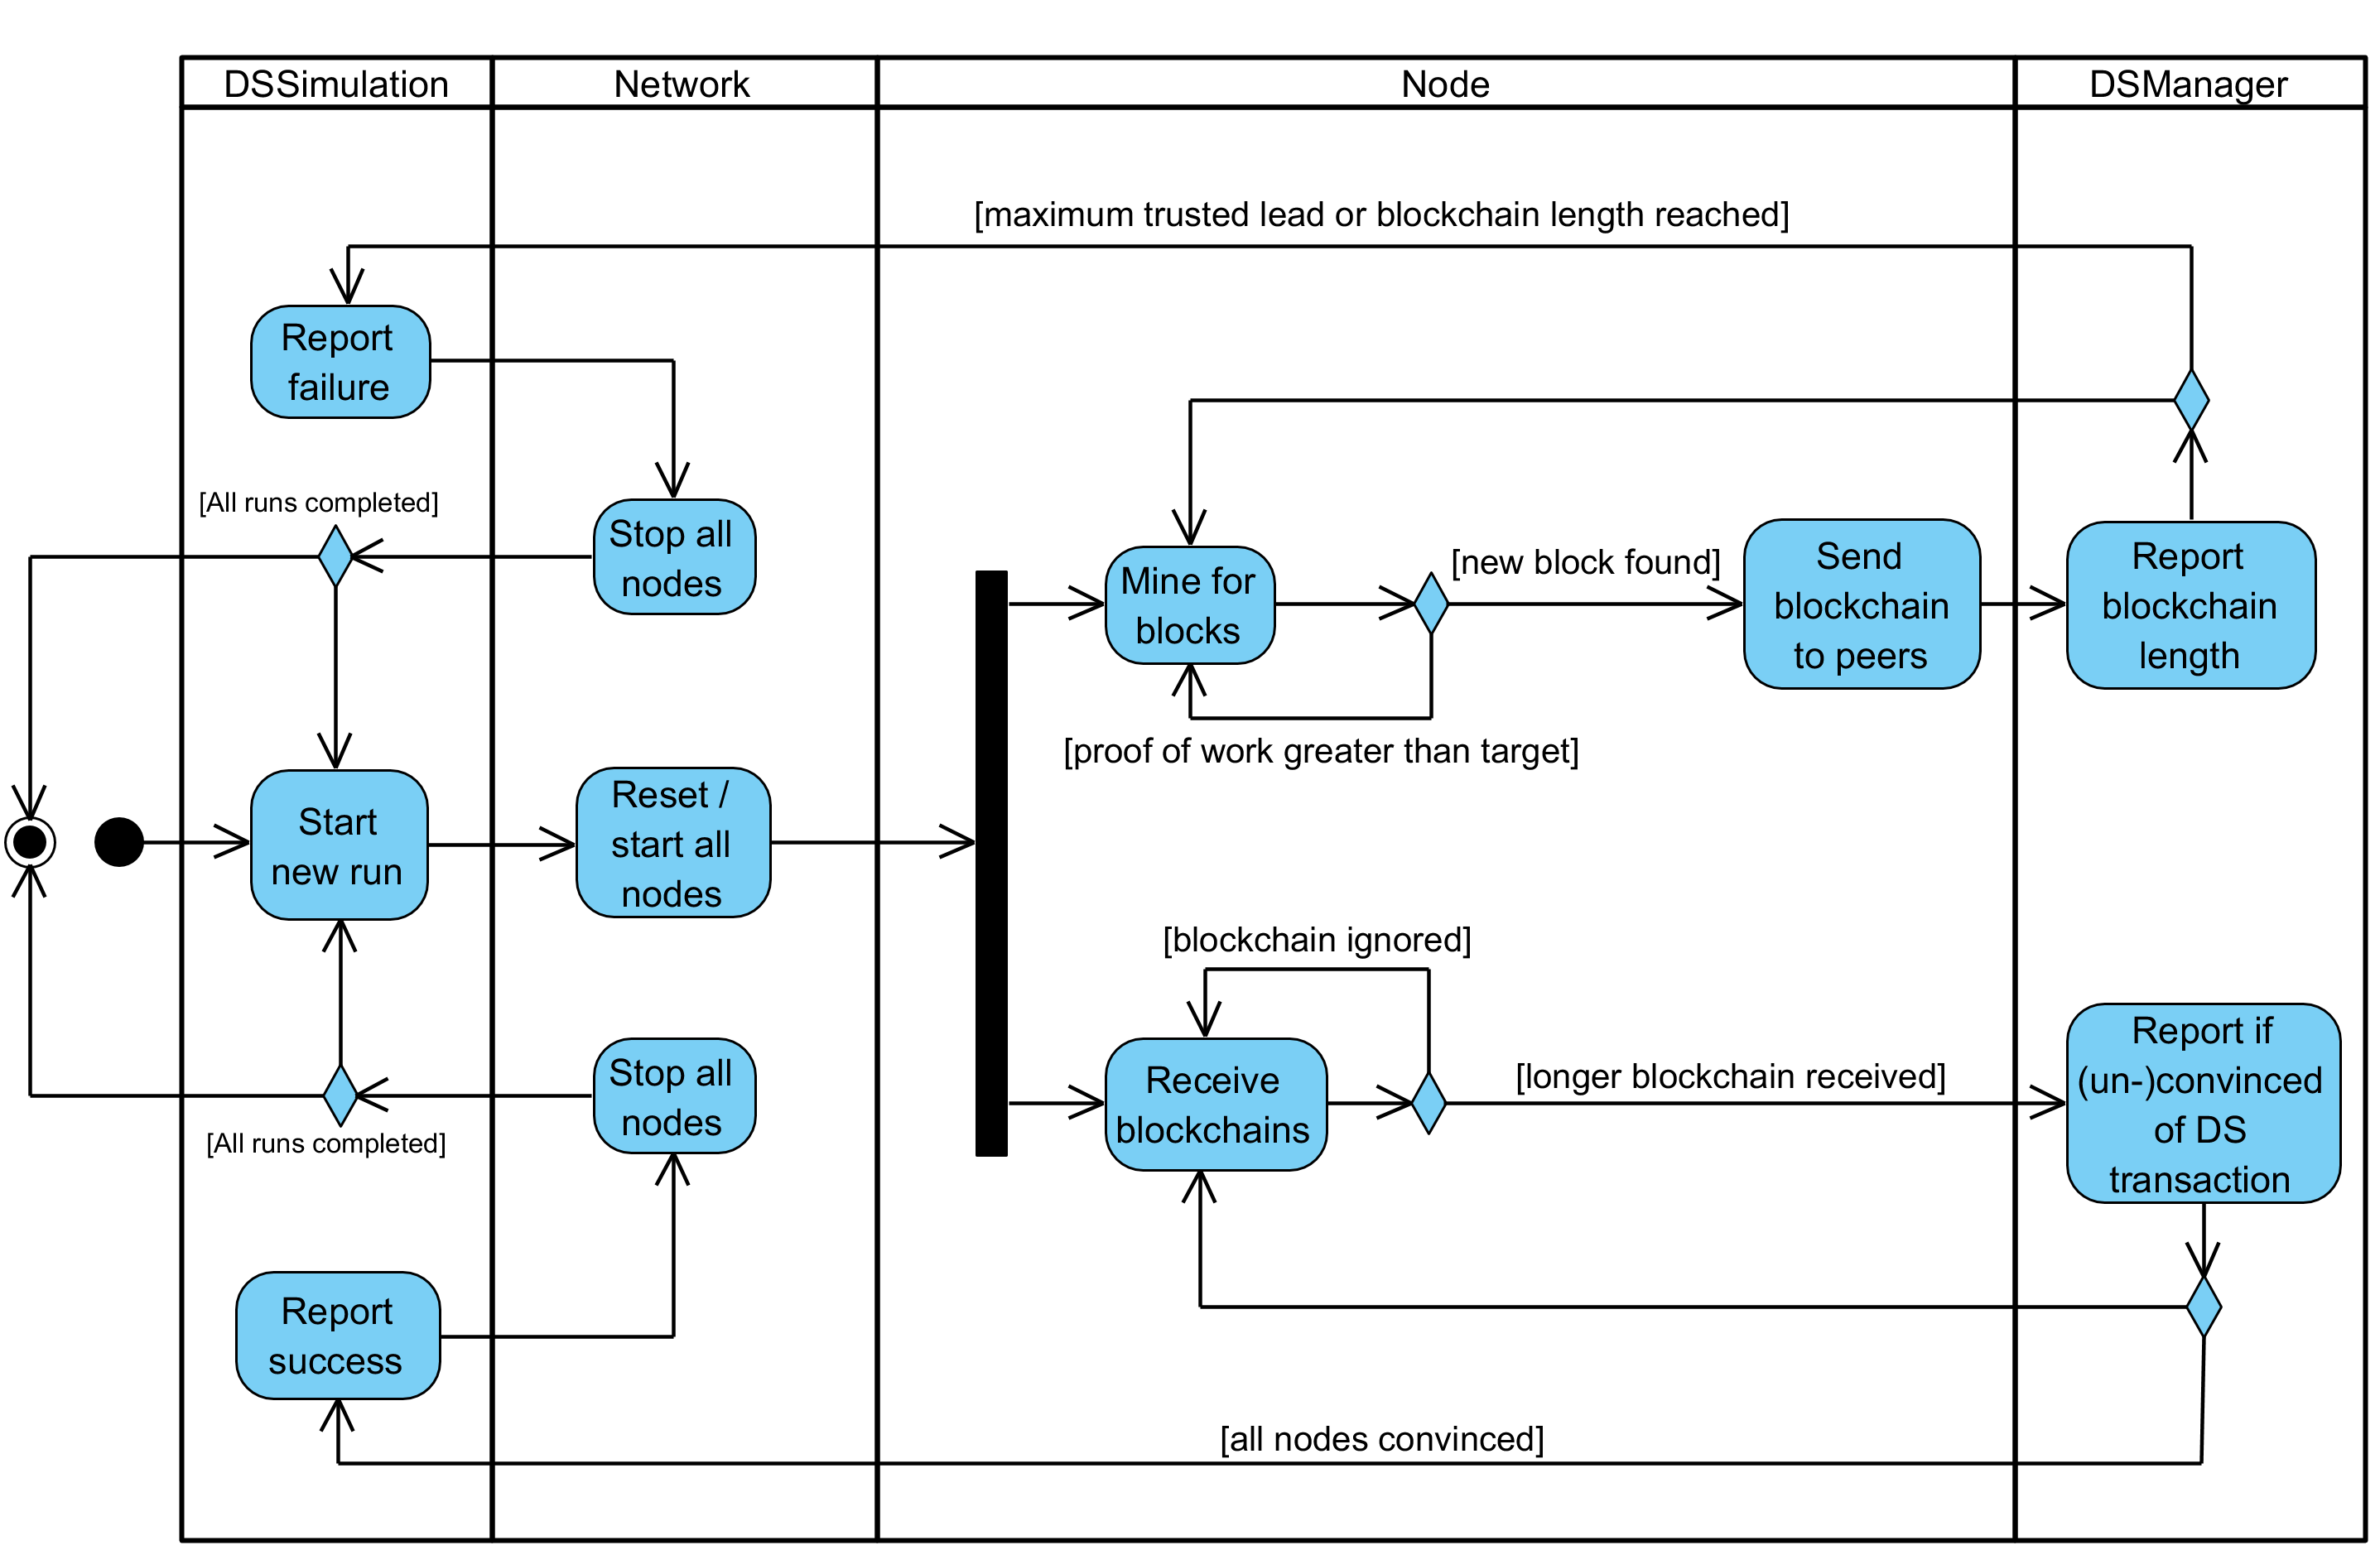
\includegraphics[width=\textwidth]{Activity1.png}
	\caption{UML activity diagram of the double-spend simulation.}
	\label{activity1}
\end{figure}

\section{Using the Simulator} \label{usage}
The \textit{DSSimulation} class is the main entry point of the double-spend simulator. It is instantiated by calling the constructor with two peer strategies to create the networks, a connection strategy to connect both networks and a parameters object. If all network strategies have been defined in the parameters object, calling the construct with just the parameters object is sufficient as well. The simulation is started by calling the simulator's \textit{start()} method. The results will be printed out onto the console after all runs have been completed. 
\subsection{Parameters} \label{params}
The parameters object is a collection of constants and variables defining the simulated conditions. All parameters can be accessed by their corresponding getter functions.
\subsubsection{Number of Nodes}
The number of nodes consists of the number of attacking and trusted nodes in the networks. Consequently, there should be at least one node in each of the networks. Since the number of nodes relates to the number of threads created by the simulator, large amounts of nodes should be considered carefully. In the following, the ratio between attacking and trusted nodes will be defined as $R$.
\subsubsection{Mining Difficulty Target}
Mining a block in the simulation requires finding a random number $x$ which is smaller than a target difficulty $T$, where $x$ is chosen from a uniform distribution between zero and one (\autoref{uniform}). By defining the target interval as shown in \autoref{tinterval}, the target difficulty precisely represents the probability of the next random number to be a valid proof of work.
\begin{subequations}
\begin{equation}\label{uniform}
x \in X\sim \mathcal{U}(0,1)
\end{equation}
\begin{equation}\label{tinterval}
T \in [0,1]
\end{equation}
\begin{equation}\label{probability}
Pr[X \leq T] = F(T) = T
\end{equation}
\end{subequations}
\subsubsection{Confirmations}
Let $C$ be the simulated number of confirmations a target merchant is waiting for before sending his product. We assume that the merchant's payment \textbf{T\textsubscript{M}} is mined into the first block of the honest blockchain, since previous blocks would be available to the attacking network as well and therefore do not influence the race between trusted and attacking blockchain forks. All nodes initially start mining on blockchains of length 0. The length of a trusted blockchain therefore indicates the number of confirmations \textbf{T\textsubscript{M}} has already received. Once this length reaches the simulated number of confirmations $C$, the merchant \textit{M} considers the payment \textbf{T\textsubscript{M}} to be valid and sends the purchased product or service to the attacker, which is assumed to be irreversible. At this point the attacker is in possession of the product and can safely begin to convince the trusted nodes of the reversed transaction \textbf{T\textsubscript{A}} by publishing the possibly longer, secret fork.
\subsubsection{Network Latency Times}
A total of three latency times are defined in the parameters object. These three parameters consist of $L_A$ defining the latency in the attacking network, $L_T$ corresponding to the trusted network's latency and $L_C$ declaring the latency between the attacking and trusted network. While $L_A$ and $L_T$ are each used by one \textit{PeerStrategy} (Section \ref{peerstratsection}) instance describing the topologies of the networks, $L_C$ is used by the \textit{ConnectionStrategy} (Section \ref{connstrat}) to model an attackers ability of sending fraudulent blockchains to the trusted network. The values represent the mean latency times in milliseconds needed to define the Gaussian distributions (Equation \ref{distribution}), in order to sample edge weights of the selected peer and network strategies.
\subsubsection{Network Graph Densities}
When using the random graph strategy (Section \ref{rndgraphstrategy}) the number of edges is defined by the graph density. The parameters object therefore allows specification of a density value for the attacking network ($D_A$) and the trusted network ($D_T$) in order to simulate discrepancies in the quality of attacking and trusted networks. The graph density is a value of the interval $[0,1]$ and represents the ratio of existing edges in a graph compared to the maximum amount of possible edges. Since the created graph has to be connected, the lowest sensible density value is $\frac{2}{n}$, where $n$ is the number of nodes in the network.
\subsubsection{Number of Double-Spend Attempts}
Using the parameters object, the number of simulation runs can be defined. One run consists of a single double-spend attempt on the modeled network which is either successful or not. By conducting several attempts, a ratio between successful and total attempts can be measured, which is the resulting value of the simulation. This measure is indicative of the trusted network's resistance against double spend attacks.
\subsubsection{Fault Tolerance}\label{faulttolerance}
To avoid the simulation running endlessly, in case the attackers are unable to gain a lead with their secret blockchain fork, it has to be defined when a simulation run can be considered as unsuccessful. This is achieved by the \textit{DSManager} class using the \textit{maximum lead} and \textit{maximum size} parameters (Section \ref{manager}). Since double spend attacks are theoretically always possible regardless of the trusted network's lead or the current blockchain length, these two parameters depend on a fault tolerance $\varepsilon$ specified in the parameters object.

Let $t$ and $a$ be the number of trusted and attacking nodes respectively and $t>a$. Using Nakamoto's probability $Q_z$ of an attacker catching up after falling $z$ blocks behind \cite{nakamoto2008bitcoin}, we define $\varepsilon$ as the minimal probability of the attacking network still being able to catch up, before the attempt is considered as unsuccessful. We then derive the maximum value of $z$ that the attackers are allowed to fall behind in order to maintain a probability $>\varepsilon$ of still catching up.
\begin{subequations}
\begin{equation}
Q_z\approx \left( \frac{a}{t} \right) ^{z} < \varepsilon
\end{equation}
\begin{equation}
z < \log_{\frac{a}{t}} \varepsilon
\end{equation}
\begin{equation}
MAX\_LEAD=\begin{cases}
    \infty, & \text{if $a\geq t$}\\
    \ceil{\log_{\frac{a}{t}} \varepsilon}, & \text{otherwise}
  \end{cases}
\end{equation}
\end{subequations}
It can be seen that if $t\leq a$, in this simplified model, the probability of an attacker catching up from a certain deficit is always one. But especially if $t= a$ and a steady lead by the trusted nodes is maintained, our simulation could still be running infinitely. Therefore, the simulation will stop in failure after a maximum blockchain length (Equation \ref{maxlength}) is reached. 
\begin{equation}\label{maxlength}
MAX\_LENGTH= \frac{1}{100\varepsilon}
\end{equation}

\subsection{ParametersBuilder}
The parameters object can be created using a \textit{ParametersBuilder}, which is offering setter functions to all available parameters. The \textit{ParametersBuilder} is an implementation of the builder pattern and can be used to instantiate the parameters object as shown in \autoref{builderlist}. Undefined parameters will be set to the default values listed in \autoref{prop}.
\begin{lstlisting}[language=Java, caption=Initializing parameters using the ParametersBuilder,label=builderlist]
ParametersBuilder b = new ParametersBuilder();
Parameters p1 = b.setTrustedNodes(40)
	.setAttackerNodes(13)
	.setAttackerPeerStrategy(PeerStrategyEnum.CONSTANT)
	.setTrustedLatency(500)
	.setConfirmations(6)
	.build();
Parameters p2 = b.setAttackerNodes(18)
	.build();
\end{lstlisting}
\subsubsection{Randomized Parameters}
The simulator and the parameters object support randomization of the confirmation, latency and density parameters. If parameters are randomized, a new value will be generated according to the specified bounds after every new simulation run. The parameters can be randomized by providing the desired inclusive lower and upper bounds to the \textit{ParametersBuilder} before building the parameters object. Parameters can be reset to specific values by calling the builder's setter function and rebuilding the object.
\begin{lstlisting}[language=Java, caption=Randomizing parameters using the ParametersBuilder]
ParametersBuilder b = new ParametersBuilder();
Parameters p = b.randomizeConfirmations(1, 10)
                .randomizeAttackerLatency(10, 50)
                .randomizeAttackerGraphDensity(0.2, 0.7)
                .build();
\end{lstlisting}
\subsubsection{Loading from Property Files}
Using the ParametersBuilder, parameters can be loaded from external property files by providing the corresponding file name and path as shown in \autoref{proplist}. A full description of the property file's structure and usage can be found in \autoref{prop}.

\begin{lstlisting}[language=Java, caption=Loading parameters from property file,label=proplist]
ParametersBuilder b = new ParametersBuilder()
Parameters p;
try {
	p = b.loadFromProperty("parameters.txt")
	     .build();
} catch (IOException ex) {
	System.err.printf("Error: %s\n", ex);
	System.exit(1);
}
\end{lstlisting}
\subsection{The Compiled Simulator}
The documented source code of the simulation framework and the double-spend simulator can be found in \cite{github}. After compilation, the uploaded double-spend simulator can be controlled by providing a property file containing the selected parameter configuration as a command line argument.
\begin{lstlisting}[caption=Launching the simulator from the command line,label=cmd]
java -jar Blockchain.jar "parameters.txt"
\end{lstlisting}
%------- chapter 5 -------

\chapter{Evaluation} \label{eval}

\section{Design} \label{design}
To identify factors affecting a blockchain architecture's resistance against double-spend attacks, we will now explore the effects of the parameters implemented in Section \ref{params} on our double-spend simulator. This will be achieved by analyzing and interpreting the results generated by the simulator over several experimentation runs. Since our model contains multiple independent variables with interval or even rational scales, a factorial experiment design is clearly out of reach. Instead, we will conduct several experiments on each individual parameter by testing a range of possible treatments. Unless otherwise stated, parameters that are not being tested during an experiment will remain fixed to their default configuration of Appendix \ref{defaultval}. 

Dependent variables of the experiments are measured by the simulator and represent the percentage of successful double-spends ($PDS$) after 100 attempts and the percentage of stale blocks generated by the attacking ($PSB_{A}$) and trusted ($PSB_{T}$) networks (Chapter \ref{simulator}). The number of stale blocks will provide additional information on blockchain dynamics and help us interpret the parameters' effects on double-spend resistance. 

The simulator is configured to use two \textit{RndGraphStrategies} (Section \ref{rndgraphstrategy}) throughout all of the experiments. Therefore, effects of the network topology will be tested by providing different treatments to the graph density parameters. Using randomization, the graphs corresponding to the attacking and trusted networks will be recreated after each double-spend attempt. 

The sampled data, representing the $PDS$, will be gathered in form of scatter plots. To provide a general trend of the data, simple exponential models of the form
\begin{equation}\label{model}
M(p) = Ae^{Bp}
\end{equation}
are fitted using non-linear regression functions of \cite{nlxb} and visualized in form of graphs for every experiment of parameter $p$. Concrete values of $A$ and $B$ for each fitted curve are listed in \autoref{modelparams}. The percentage of stale blocks ($PSB$) is modeled and visualized using LOESS-fits \cite{loess,r}. 

The goal is to provide evidence that each of the model's independent variables does in fact have an impact on $PDS$. To achieve this, the generated data will be tested against null hypotheses of the form

\begin{itemize}
\item[] $H_{0,p}$ : Parameter $p$ has no effect on $PDS$,
\end{itemize}
using the Kruskal-Wallis rank sum test \cite{kruskal,r} and a confidence level of 95\%. Since 100 $PDS$ is the maximal value returned by the simulator, consecutive data points of 100 $PDS$ will be ignored in the generation of fitted curves. To receive the actual value of $PDS$ when applying one of the fitted models, the model's formula can instead be altered to
\begin{equation}\label{min}
PDS = min(M(p), 100).
\end{equation}
\section{Results} \label{results}
\subsubsection{Number of Nodes $N$}
To determine whether the total number of nodes in the network has an effect on the $PDS$, multiple simulations have been run while gradually raising the number of nodes in both networks. By increasing the number of attacking nodes by 30 and the number of trusted nodes by 60, the ratio between attacking and trusted nodes remains at a constant level of $\frac{1}{3}$. Runs for each treatment have been replicated five times. \autoref{numnodes} represents the sampled data using a box plot, visualizing treatment levels up to 990 nodes in total.
\begin{figure}
\centering
\begin{minipage}{.5\textwidth}
  \centering
  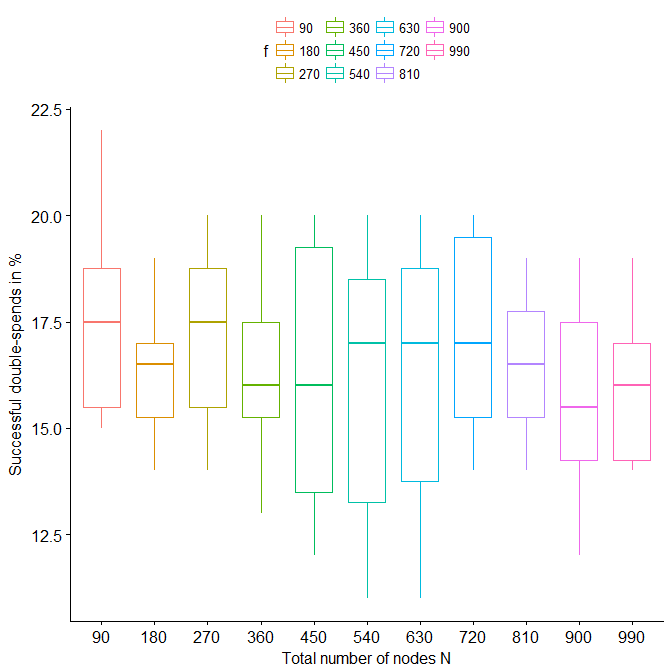
\includegraphics[width=\linewidth]{Experiments/numnodes.png}
  \captionof{figure}{Box plot of $PDS$ as \\ a function of $N$}
  \label{numnodes}
\end{minipage}%
\begin{minipage}{.5\textwidth}
  \centering
  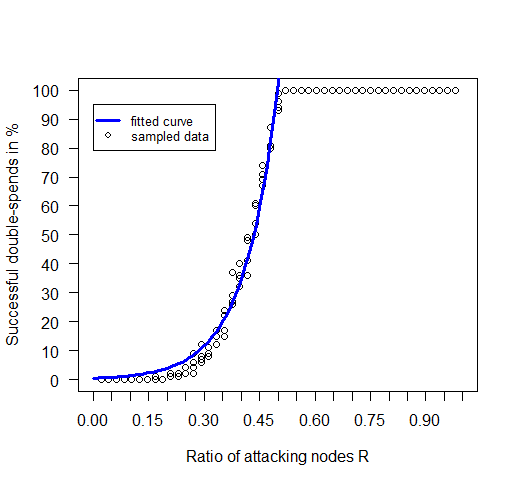
\includegraphics[width=\linewidth]{Experiments/Ratio/ratio_f.png}
  \captionof{figure}{$PDS$ as a function of\\$R$ (reference model)}
  \label{ratio}
\end{minipage}
\end{figure}

\subsubsection{Ratio of Attacking Nodes $R$}
In order to improve comparability of our results to existing work, especially hashrate-based models presented by \cite{HBDSA} and \cite{DSAwithTime} (Chapter \ref{relatedwork}), we combine the two independent variables corresponding to the number of attacking and trusted nodes into a single variable indicating the ratio of attacking nodes. Since all simulated nodes possess the same computing power, the ratio $R$ relates to the hashrate controlled by an attacker in \cite{nakamoto2008bitcoin,HBDSA,DSAwithTime}. \autoref{ratio} shows the $PDS$ as a function of the attacker ratio. Using the default configuration of \autoref{prop}, $R$ is increased by $\frac{1}{48}$ after four repetitions of 100 double-spend attempts. The resulting model will be used as a reference model in all following experiments, represented by a black curve in the plotted graphs. The proportion of hashing power required to be controlled by an attacker in order to carry out DSAs seems to be of special interest in literature. The comparison of our results with the reference model therefore enables us to visualize the influence of other parameters on the effective impact of this proportion $R$.

\subsubsection{Confirmation length $C$} \label{consres}
The confirmation length $C$ describes the number of blocks the targeted merchant is waiting for until a received payment is considered to be valid. The parameter's effect on RADS is studied in several experiments testing treatments in the range of 0 to 30 confirmations. \autoref{conf:a} shows the results of experiments with 10, 16 and 22 attacking nodes as a function of $C$. \autoref{conf:b} replicates our second experiment by testing the attacker ratio $R$ with different confirmation lengths to compare with our reference model.

\subsubsection{Connection Latency $L_C$}
Since the simulator uses the \textit{ConstantConnectionStrategy} presented in Section \ref{connstrat}, $L_C$ represents the mean latency time in milliseconds it takes until all trusted nodes receive a new block published by an attacking node. The effects of this independent variable were tested by incrementing $L_C$ by 25 milliseconds after 3 simulation runs. \autoref{conn:a} visualizes the experiments up to 700 milliseconds, while \autoref{conn:b} again shows the impact of $L_C$ on an attacker's $PDS$ when controlling a proportion $R$ of the total nodes.
\begin{figure}[ht!]
\centering
\begin{subfigure}{.5\textwidth}
  \centering
  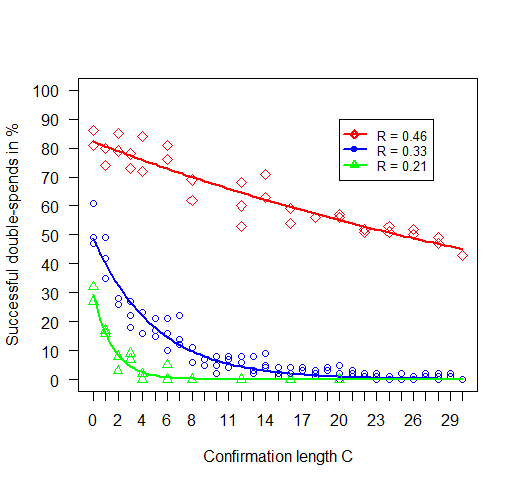
\includegraphics[width=\linewidth]{Experiments/Confirmations/conf.png}
  \caption{$PDS$ as a function of $C$}
  \label{conf:a}
\end{subfigure}%
\begin{subfigure}{.5\textwidth}
  \centering
  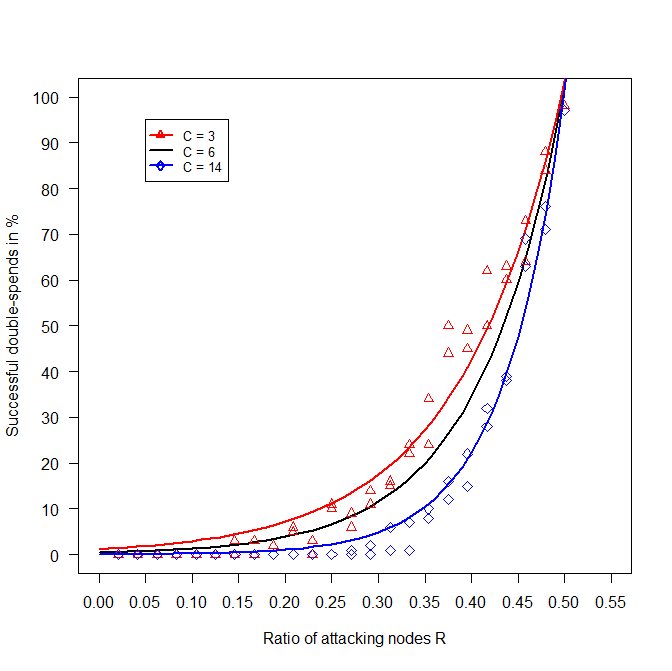
\includegraphics[width=\linewidth]{Experiments/Confirmations/confrat.png}
  \caption{$PDS$ as function of $R$ for different $C$}
  \label{conf:b}
\end{subfigure}
\caption{Effects of the confirmation length $C$ on $PDS$}
\label{conf}
\end{figure}
\begin{figure}[h!]
\centering
\begin{subfigure}{.5\textwidth}
  \centering
  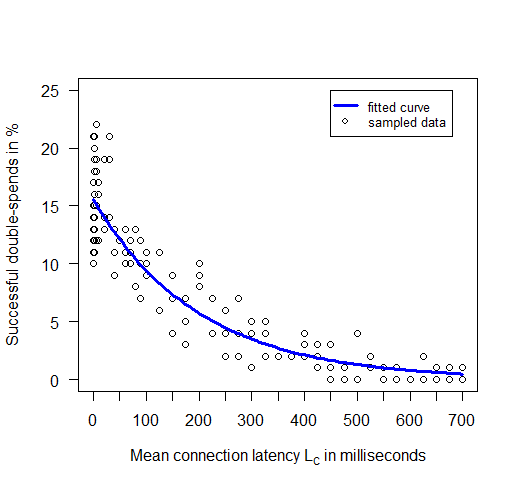
\includegraphics[width=\linewidth]{Experiments/ConnLatency/connection.png}
  \caption{$PDS$ as a function of $L_{C}$}
  \label{conn:a}
\end{subfigure}%
\begin{subfigure}{.5\textwidth}
  \centering
  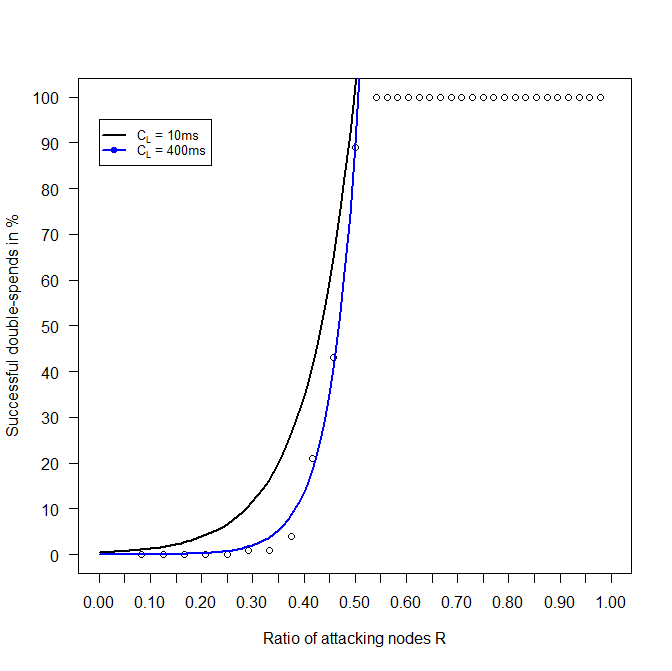
\includegraphics[width=\linewidth]{Experiments/ConnLatency/conrat.png}
  \caption{Effects of $L_{C}$ on reference model}
  \label{conn:b}
\end{subfigure}
\caption{Effects of the mean connection latency $L_{C}$ on $PDS$}
\label{conn}
\end{figure}

\subsubsection{Network Latency Times $L_{A},L_T$}
\autoref{trulat:a} shows the $PDS$ as a function of the mean latency ($L_T$) between adjacent peers in the trusted network. Effects of the parameters are tested for treatments up to 100 milliseconds, with treatment levels incremented by 5 milliseconds after 4 simulation runs. Since data points corresponding to $L_T > 75ms$ are very close to the simulator's maximal value, they are rounded up to 100 $PDS$ and ignored during the generation of the exponential model. This improves the approximation of the data, since the actual value of $PDS$ is calculated from the model as shown in Equation \ref{min}. \autoref{trulat:a} also visualizes the percentage of stale blocks generated by the trusted network ($PSB_T$) as a LOESS-fit. \autoref{trulat:b} shows the effect of different values of $L_T$ on our reference model.

\autoref{attlat:a} and \autoref{attlat:b} represent replications of the experiments testing $L_T$. The same treatments are now applied on the independent variable $L_A$, representing the mean latency between peers of the attacking network.
\begin{figure}[!ht]
\centering
\begin{subfigure}{.481\textwidth}
  \centering
  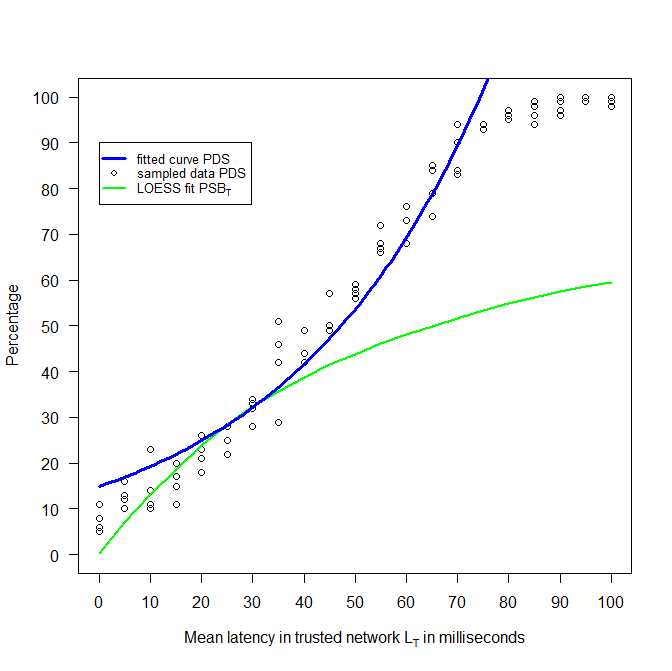
\includegraphics[width=\linewidth]{Experiments/TruLatency/trulat.png}
  \caption{$PDS$ as a function of $L_{T}$}
  \label{trulat:a}
\end{subfigure}%
\begin{subfigure}{.481\textwidth}
  \centering
  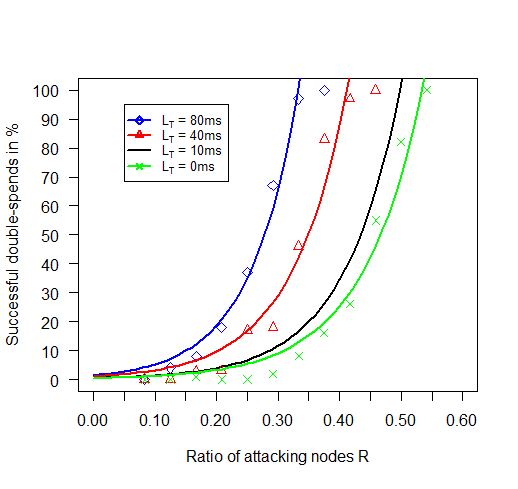
\includegraphics[width=\linewidth]{Experiments/TruLatency/trurat.png}
  \caption{Effects of $L_{T}$ on reference model}
  \label{trulat:b}
\end{subfigure}
\begin{subfigure}{.481\textwidth}
  \centering
  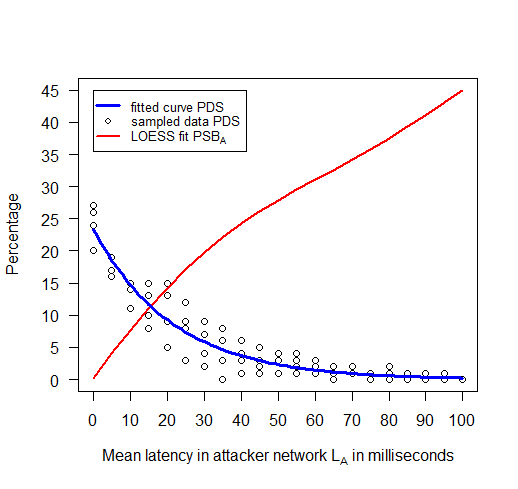
\includegraphics[width=\linewidth]{Experiments/AttLatency/attlat.png}
  \caption{$PDS$ as a function of $L_{A}$}
  \label{attlat:a}
\end{subfigure}%
\begin{subfigure}{.481\textwidth}
  \centering
  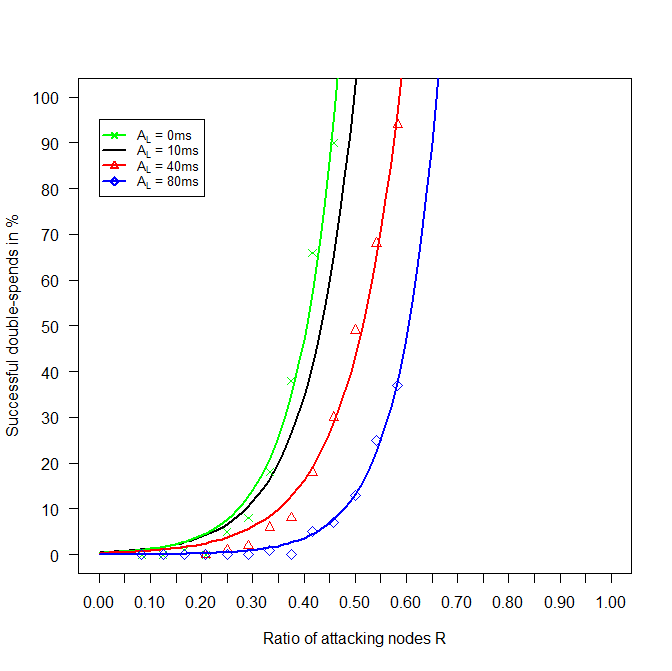
\includegraphics[width=\linewidth]{Experiments/AttLatency/attrat.png}
  \caption{Effects of $L_{A}$ on reference model}
  \label{attlat:b}
\end{subfigure}
\caption{Effects of mean trusted ($L_{T}$) and attacker ($L_{A}$) latency on $PDS$}
\label{latplot}
\end{figure}
\subsubsection{Graph Density $D_{A},D_T$}
\autoref{trudens:a} shows the $PDS$ as a function of the trusted network's graph density. Two experiments with network latency times of 10ms and 100ms are conducted, while the first experiment also measures the effects of the graph density on $PSB_T$. \autoref{trudens:b} shows the effect of a low trusted graph density on $PDS$ as a function of $R$, where $L_{AT}$ indicates $L_{A} = L_{T}$.

In \autoref{attdens:a} and \autoref{attdens:b}, the same experiments are replicated for the graph density in the attacker's network ($D_{A})$.

\begin{figure}[!ht]
\centering
\begin{subfigure}{.5\textwidth}
  \centering
  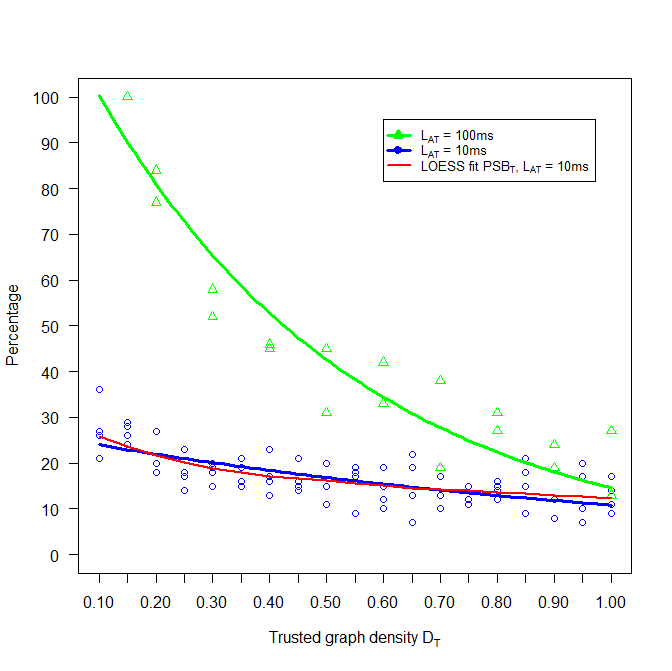
\includegraphics[width=\linewidth]{Experiments/TruDensity/trudens.png}
  \caption{$PDS$ as a function of $D_{T}$}
  \label{trudens:a}
\end{subfigure}%
\begin{subfigure}{.5\textwidth}
  \centering
  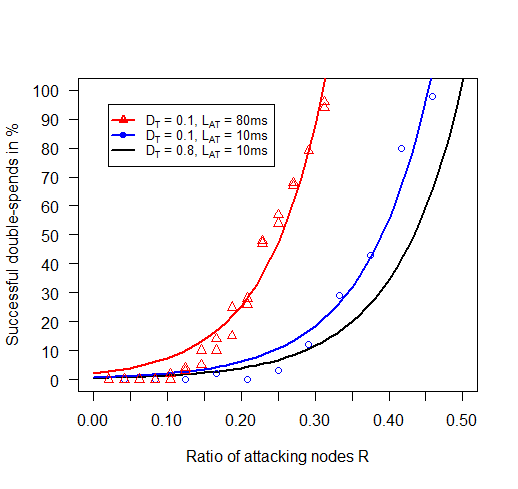
\includegraphics[width=\linewidth]{Experiments/TruDensity/trudensrat.png}
  \caption{Effects of $D_{T}$ on reference model}
  \label{trudens:b}
\end{subfigure}
\begin{subfigure}{.5\textwidth}
  \centering
  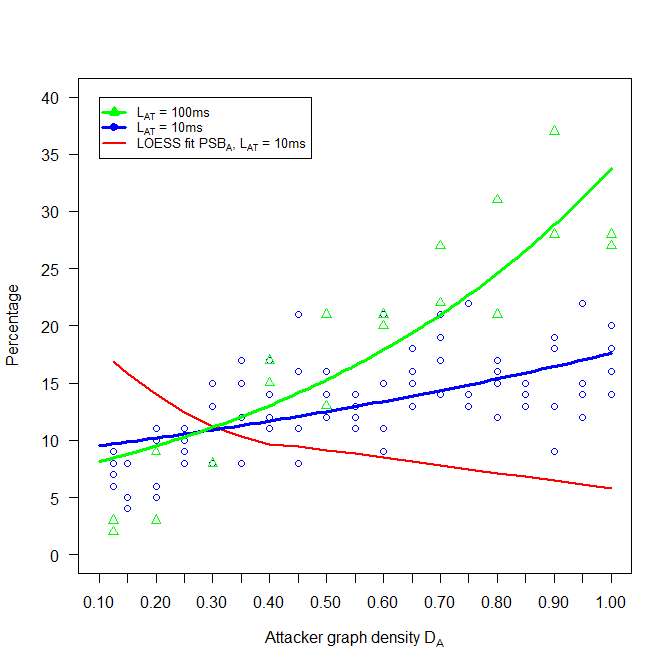
\includegraphics[width=\linewidth]{Experiments/AttDensity/attdens.png}
  \caption{$PDS$ as a function of $D_{A}$}
  \label{attdens:a}
\end{subfigure}%
\begin{subfigure}{.5\textwidth}
  \centering
  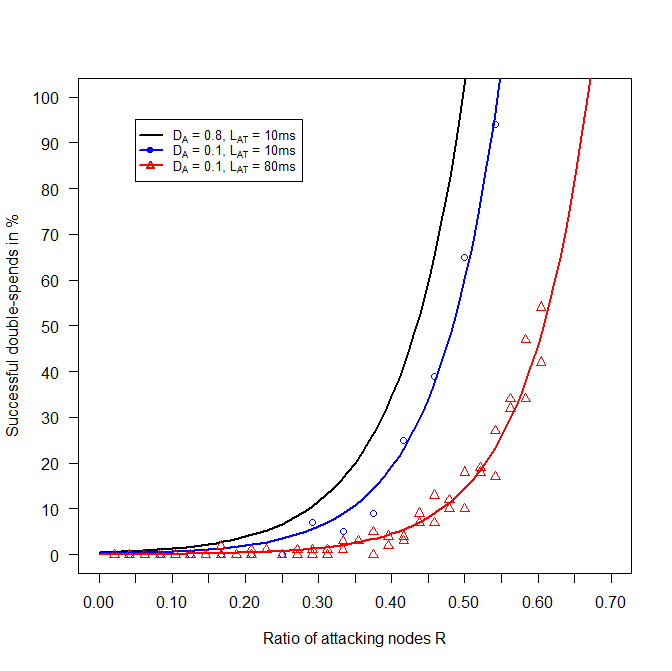
\includegraphics[width=\linewidth]{Experiments/AttDensity/attdensrat.png}
  \caption{Effects of $D_{A}$ on reference model}
  \label{attdens:b}
\end{subfigure}
\caption{Effects of trusted ($D_{T}$) and attacker ($D_{A}$) graph density on $PDS$}
\label{densplot}
\end{figure}

\subsubsection{Difficulty target $T$}
\autoref{diff:a} represents the $PDS$ as a function of the difficulty target $T$, while also indicating the rise of $PSB$ in both networks when increasing the target. Note the logarithmic scale of the axis representing $T$. \autoref{diff:b} compares different combinations of difficulty targets and latency times in both networks to our reference model, where $L_{AT}$ again indicates $L_{A} = L_{T}$.\begin{figure}[hb!]
\centering
\begin{subfigure}{.5\textwidth}
  \centering
  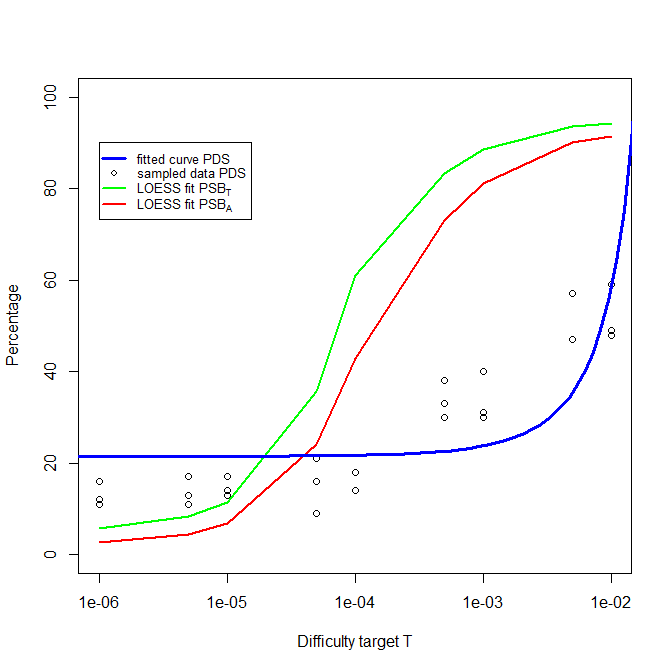
\includegraphics[width=\linewidth]{Experiments/Difficulty/difficultyfit.png}
  \caption{$PDS$ and $PSB_{A,T}$ as functions of \\ $T$ on logarithmic scale}
  \label{diff:a}
\end{subfigure}%
\begin{subfigure}{.5\textwidth}
  \centering
  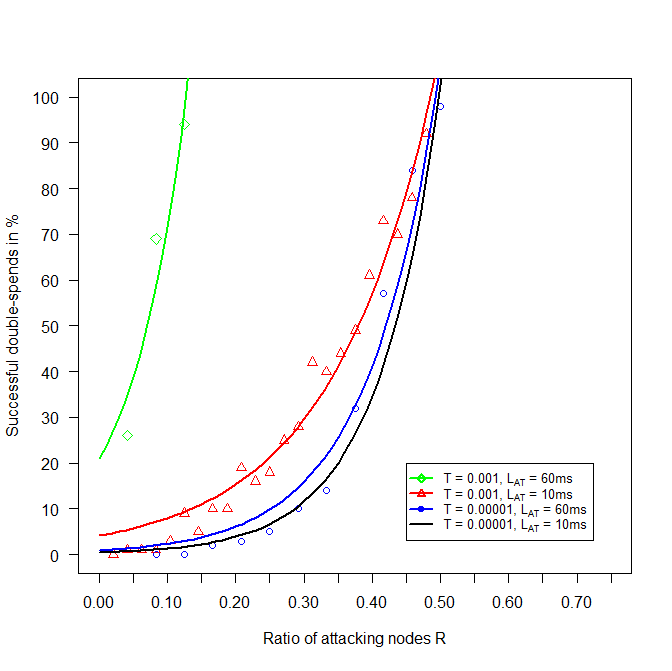
\includegraphics[width=\linewidth]{Experiments/Difficulty/diffrat.png}
  \caption{Effects of different combinations of \\ $T$ and $L_{A,T}$ on reference model}
  \label{diff:b}
\end{subfigure}
\caption{Effects of the difficulty target $T$ on $PDS$}
\label{diff}
\end{figure}

\section{Discussion} \label{discussion}
\subsubsection{Number of Nodes $N$}
\autoref{numnodes} suggests that the means of the factor levels for $N$ are roughly equal and no underlying trend of the data can be observed immediately. This assumption is validated by the Kruskal-Wallis test in \autoref{nanova}. Since $p > 5\%$, the differences in the means of factor levels are not significant at a level of 5\%. Therefore, the null hypothesis $H_{0,N}$, as defined in Section \ref{design}, can not be rejected. We conclude that the amount of total nodes $N$ has no significant effect on $PDS$. Since all nodes of the simulator possess the same computing power, this observation is sensible. We assume that especially the proportion of attacking nodes compared to trusted nodes results in a change of $PDS$. As this proportion was kept at a constant level in \autoref{numnodes}, no effects can be observed.
\begin{table}[ht]
\centering
\begin{tabular}{|l|l|l|l|l|l|} \hline
& Df & $\chi^{2}$ & p-value \\ \hline
$N$ & 10 &  2.7562 & 0.9866 \\ \hline
\end{tabular}
\caption{Results of Kruskal-Wallis test for $H_{0,N}$}
\label{nanova}
\end{table}
\subsubsection{Ratio of Attacking Nodes $R$}
The trend of \autoref{ratio} is comparable to the plots of hashrate-based models by \cite{HBDSA} or \cite{DSAwithTime}, whereas the hashrate possessed by an attacker corresponds to the ratio of nodes under an attacker's control in our model. The $PDS$ seems to be rising exponentially with increasing $R$, which is also confirmed by the fitted curve. Once the majority of the network is controlled by an attacker, double-spend attacks appear to be always successful. An important difference and interesting observation is that at exactly 50\% control of the attacker successful DSAs are not guaranteed. This observation is contrary to the mathematical models proposed by \cite{nakamoto2008bitcoin,HBDSA,DSAwithTime} and might be a result of the network parameters, whose effects have not been evaluated at this point. Another reason of this observation could be seen in the end conditions of our simulator. If the trusted network is able to maintain a steady lead over the attackers' blockchain fork without triggering the maximum lead parameter to end the simulation, the attempt will fail after a maximum blockchain length is reached. This scenario is especially likely if the attacking network's computing power is very similar to the computing power controlled by the trusted nodes, since this results in both networks having equal chances of mining the next block. In reality, this observation might correspond to an attacker being unable to maintain the necessary resources of conducting a DSA over a long timeframe. The attacker might be forced to abort the DSA, since mining on a secret chain does not generate any revenue. \cite{longestchain} argues in a similar way, in that an attacker will only be able to maintain such a significant amount of hashing power over a short period of time. 

According to \autoref{ranova} and the observable pattern in \autoref{ratio}, the differences between data means are significant at a level of 5\%. We therefore successfully reject $H_{0,R}$.
\begin{table}[hb]
\centering
\begin{tabular}{|l|l|l|l|l|l|} \hline
& Df & $\chi^{2}$ & p-value \\ \hline
$R$ & 46 & 164.69 & 2.909e-15 \\ \hline
\end{tabular}
\caption{Results of Kruskal-Wallis test for $H_{0,R}$}
\label{ranova}
\end{table}
\subsubsection{Confirmation length $C$} \label{consdisc}
According to \autoref{conf:a}, an increasing amount of confirmations successfully reduces the $PDS$ as intended by the protocol. Regardless, the effect decreases significantly with increasing $R$ and, looking at \autoref{conf:b}, the confirmation length has no effect at all once an attacker gains control over the majority of computing power in the network. This observation seems plausible and confirms the results of \cite{nakamoto2008bitcoin,HBDSA}, describing that every trusted lead can be overcome by an attacker once the majority is mining on the malicious chain. Overall, a merchant should aim to wait for as many confirmations as possible in order to reduce the risk of double-spend attacks. The concrete amount of confirmations could be determined by the value of the merchant's product.

Combining the data of the three plots in \autoref{conf:a} enables us to perform a Kruskal-Wallis test (\autoref{canova}). Using the generated results, we successfully reject $H_{0,C}$ at a significance level of 5\%.
\begin{table}[hb]
\centering
\begin{tabular}{|l|l|l|l|l|l|} \hline
& Df & $\chi^{2}$ & p-value \\ \hline
$C$ & 30 & 81.106 & 1.368e-06 \\ \hline
\end{tabular}
\caption{Results of Kruskal-Wallis test for $H_{0,C}$}
\label{canova}
\end{table}
\subsubsection{Connection Latency $L_C$} \label{connlatsec}
At the first glance, effects of increasing the connection latency $L_C$ seem to be similar to an increase in the confirmation length. The $PDS$ is reduced by longer latency times, but once an attacking ratio of 50\% is reached, the parameter shows no effect (\autoref{conn:b}). This phenomenon can be explained by regarding the nature of the connection latency. Assume Alice plans a DSA and experiences a latency time of $L_C$ to every trusted node. For her attack to be successful, she needs to gain a sufficient lead with her secret blockchain branch in order to still be ahead of the trusted nodes' chain once her malicious branch reaches the targeted network. During $L_C$ the trusted network might be able to catch up to Alice's branch, despite her possibly being in the lead at the time she sent her copy. However, if Alice controls more computing power than the defending network, she will always be able to generate an arbitrarily large lead over the trusted nodes' chain, thereby successfully overcoming $L_C$. The connection latency could be increased by the trusted network by not revealing concrete addresses of peers in order to hide them from potential attackers and be more resistant against double-spend attacks. An attacker will always aim to gather as much information as possible about trusted peers to reduce the maximum $L_C$.

The Kruskal-Wallis test results in \autoref{conanova} indicate that $L_C$ does in fact have a significant effect on $PDS$, allowing us to reject $H_{0,L_C}$ at our confidence level of 95\%.
\begin{table}[hb]
\centering
\begin{tabular}{|l|l|l|l|l|l|} \hline
& Df & $\chi^{2}$ & p-value \\ \hline
$L_C$ & 37 &  120.36 & 9.409e-11 \\ \hline
\end{tabular}
\caption{Results of Kruskal-Wallis test for $H_{0,L_C}$}
\label{conanova}
\end{table}
\subsubsection{Network Latency Times $L_{A},L_T$}
The visible effects of $L_{A}$ and $L_{T}$ on $PDS$ in \autoref{latplot} can be explained by observing the percentage of stale blocks generated during the experiments. At 0 milliseconds of latency between peers no stale blocks are mined. This is plausible since block propagation is instant and the participating nodes are in consent at all times. However, with increasing latency times, chances of two nodes mining a block before being notified by each other increase as well, therefore raising the amount of stale blocks. As stale blocks do not contribute to the length of the consented blockchain, their creation indicates a waste of computing power, especially when defending against double-spend attacks. Networks with high $PSB$ consequently possess less \textit{effective} computing power than networks with a lower $PSB$ and the same number of nodes (hashrate). \autoref{attlat:a} shows how an increase in $L_{A}$ raises $PSB_A$, which in turn reduces the effective computing power possessed by the attacking network, resulting in a lower $PDS$. Since the distribution of computing power is represented by $R$ in our model, a translation along the $R$-axis for different $L_{A}$ can be observed in \autoref{attlat:b}. Consequently, an increase in $L_{A}$ leads to the decrease of $R$, whereas an increase in $L_{T}$ corresponds to an increase in $R$. We conclude that it is not sufficient to only consider the number of nodes or the hashrate controlled by each network when analyzing the distribution of computing power between attacking and defending networks. Instead, it is also important to consider how well nodes of a network are working together on a single consented blockchain and how many hashes are wasted towards the computation of stale blocks. The $PSB$ is therefore indicative of a network's mining efficiency which is affecting their capability of extending the blockchain. 

To maximize resistance against double-spend attacks the trusted network should aim to reduce the overall latency in their network. It should also be considered that an attacker might use the same infrastructure and protocol as the trusted nodes. Additionally, the attacker might deliberately target the trusted node's communication with other attacks in order to increase $L_{T}$ and consequently the chance of double-spend attacks.

The results of the Kruskal-Wallis tests in \autoref{latanova} allow us to successfully reject $H_{0,L_A}$ and $H_{0,L_T}$ at a confidence level of 95\%, confirming the significant effect of the parameters on $PDS$.
\begin{table}[hb]
\centering
\begin{tabular}{|l|l|l|l|l|l|} \hline
& Df & $\chi^{2}$ & p-value \\ \hline
$L_A$ & 20 &  70.515 & 1.501e-07 \\ \hline
$L_T$ & 20 &  81.603 & 2.095e-09 \\ \hline
\end{tabular}
\caption{Results of Kruskal-Wallis test for $H_{0,L_A}$ and $H_{0,L_T}$}
\label{latanova}
\end{table}

\subsubsection{Graph Density $D_{A},D_T$}
Similar to $L_{A}$ and $L_{T}$, the graph density influences the amount of stale blocks mined by the networks, producing comparable effects on $PDS$. A network with low graph density contains less edges between nodes, which increases the average latency time between peers. Nodes of dense networks consequently work together in higher harmony, resulting in less computational power being wasted towards the mining of stale blocks. Therefore, denser networks excel at extending their consented blockchain by increasing efficiency of sharing new blocks. Again, the effects on the functions of $R$ in \autoref{trudens:b} and \autoref{attdens:b} can be roughly described as a translation along the $R$-axis. An important observation can be seen in the fact that a higher latency time appears to amplify the effects of the graph density on $PDS$ and vice versa. This is plausible, since adding edges to a high latency network reduces overall latencies to a higher degree compared to adding edges in an already low latency network. To increase resistance against DSAs, the trusted network should gather information about as many peers as possible in order to increase density of the network and reduce latency times. This might again be influenced by an attacker using denial of service or similar attacks on the nodes' communication.

The results of performing two Kruskal-Wallis tests on the data of \autoref{trudens:a} and \autoref{attdens:a} are listed in \autoref{densanova}. Since both $p$-values are below 5\%, the graph density can be considered to have a significant effect on $PDS$. We conclude in rejecting $H_{0,D_A}$ and $H_{0,D_T}$.
\begin{table}[h!]
\centering
\begin{tabular}{|l|l|l|l|l|l|} \hline
& Df & $\chi^{2}$ & p-value \\ \hline
$D_A$ & 18 &  57.391 & 5.364e-06 \\ \hline
$D_T$ & 18 & 34.8 & 0.01001 \\ \hline
\end{tabular}
\caption{Results of Kruskal-Wallis test for $H_{0,D_A}$ and $H_{0,D_T}$}
\label{densanova}
\end{table}

\subsubsection{Difficulty target $T$} \label{diffanalysis}
The effects of changing the difficulty target $T$ are again closely related to the amount of stale blocks generated by the attacking and trusted networks. If $T$ is small, chances of finding a valid proof of work decline as well, making it more difficult to mine a new block. This results in less blocks being mined on average, which decreases the chances of two blocks being mined at roughly the same time creating a stale block. If $T$ is increased, more blocks are mined overall, resulting in a higher percentage of stale blocks. \autoref{diff:a} shows the $PSB$ of both networks as a function of $T$. At the lowest tested difficulty target barely any stale blocks are created. However, after raising the target, over 90\% of all blocks generated by both networks are stale. Since $PSB_A$ and $PSB_T$ are comparably high, both networks are wasting similar amounts of computing power on the creation of stale blocks. But despite both networks being equally affected by the high $PSB$, the attacking networks seems to benefit in their attempts of double-spend attacks. Because of the outstanding majority of blocks being stale, each node in the networks is effectively mining on its own. Only rarely will a node receive blockchains longer than its own copy, since latency times are too long in relation to the difficulty target and the node has already mined more blocks on its own chain when receiving its peers' blockchains. If each node is mining on its own, the computing power of the attacking and trusted networks consists of effectively one node. In the worst case, this leads to 50\% of the computing power being controlled by an attacker, increasing the chance for DSAs significantly.

Effects of the difficulty target are obviously always related to the latencies in the networks. We therefore distinguish between \textit{high} difficulty targets, leading to high amounts of stale blocks and vulnerability against DSAs and \textit{low} difficulty targets leading to a lower $PSB$ and therefore higher resistance against DSAs. More specifically, a low difficulty target in a low latency network could resemble a high difficulty target in a high latency network, since more stale blocks will be generated. Ultimately, the difficulty target should always be chosen in a way resulting in the least amount of stale blocks and therefore maximum collusion between nodes.

\autoref{diff:b} visualizes the relation between latency and difficulty targets. While increasing the latency mean in both networks by 50 milliseconds at a difficulty target of 0.00001 has almost no effect on $PDS$, increasing the latency at $T$ = 0.001 leads to a significantly higher amount of successful DSAs. While 0.001 might be considered a low difficulty target at a mean latency of 10 milliseconds, it is not low enough in networks experiencing higher latencies. 

The goal of the trusted network is to increase resistance against double-spend attacks. Therefore, it would be advantageous to establish a low difficulty target in regards to the latency and density of their network. Since these network parameters often depend on communication architecture or hardware they might be hard to influence. However, by choosing a suitable difficulty target, deficits in $L_{T}$ and $D_{T}$ might be compensated, maximizing collusion and consent between nodes.

The significance of the difficulty target $T$ in regards to $PDS$ is validated by the Kruskal-Wallis test in \autoref{tanova}, allowing us to reject $H_{0,T}$
\begin{table}[hb]
\centering
\begin{tabular}{|l|l|l|l|l|l|} \hline
& Df & $\chi^{2}$ & p-value \\ \hline
$T$ & 8 &  21.637 & 0.005634 \\ \hline
\end{tabular}
\caption{Results of Kruskal-Wallis test for $H_{0,T}$}
\label{tanova}
\end{table}

\section{Limitations} \label{limits}
Although simulations and experiments are generally accepted as ways to analyze
and explore the behavior of diverse and dynamic systems, limitations of our results should be mentioned. During development of the simulator, simulation runs and the generation of results, some threats to the validity of our experiments were identified which will be summarized in the following sections. 
\subsubsection{Miner Scheduling}
The simulation runs were carried out on two machines using \textit{Windows 7} and \textit{Ubuntu 16.04} operating systems equipped with \textit{Intel i5} processors. Since each miner is represented by a single thread, scheduling was required to simulate concurrency. Throughout the experiments it was realized that sometimes certain mining threads were given access to the processing unit for too long, resulting in multiple blocks being mined by a single node before other nodes were given the chance to generate a proof of work. This phenomenon is especially relevant during simulations of high difficulty targets, which leads to many blocks being mined in quick succession. Although access to the processing unit between trusted and attacking nodes converges over time, some nodes were able to generate a significant advantage by generating multiple blocks early during the simulation run. This issue has been addressed by synchronizing the mining threads after each node has generated 10 random numbers towards their next proof of work. This way, each node can only generate a maximum of 10 random numbers ahead of its peers, reducing the likelihood of multiple blocks due to the scheduling bias. Nevertheless, the phenomenon might still persist, especially when simulating very high difficulty targets ($T > 0.1$).
\subsubsection{Constant Connection Strategy}
The only implemented and tested connection strategy is the \textit{ConstantConnectionStrategy} presented in Section \ref{connstrat}. This strategy assumes that each attacking nodes is aware of every trusted node in the system and manages to establish a connection of constant latency to all targeted nodes. Although this is the optimal strategy an attacker should strife for, since it reduces the time needed to send fraudulent blockchains to the trusted nodes, some trusted peers could be masked by the network and unknown to an attacker. A connection strategy using a \textit{connection density} parameter is missing in our simulation, therefore such a scenario was not examined. It is assumed that reducing the density of an attacker's connection to the trusted network produces similar effects as increasing the connection latency $L_C$.
\subsubsection{Random Graph Creation}
The pseudo-random graph created by the \textit{RndGraphStrategy} in Section \ref{rndgraphstrategy} is not perfectly random. The strategy makes use of Algorithm \ref{rndgraph}, which introduces a bias to certain topologies. The algorithm initially creates a pseudo-random spanning tree of $n-1$ edges and $n$ nodes by iterating through all nodes in the network. During each iteration, a random node of already visited and connected nodes is chosen to create an edge with a new node, which is not yet included in the graph. Since for each iteration only visited nodes are considered for one end of a new edge, earlier nodes are more likely to receive a higher degree. This could alter effects of parameters regarding the network topology, especially latency and graph density. Nevertheless, these effects are assumed to not be significant. Arguably, the proposed algorithm instead creates graphs that are more closely related to real computer networks by increasing the likelihood of graphs with centralized nodes \cite{stackoverflow}.
\subsubsection{Post-Hoc Analysis}
The null hypotheses formulated in Section \ref{design} were tested using the Kruskal-Wallis rank sum test. The results of this test only confirm the existence of a significant difference between groups of the same treatment level, but do not explain which specific pairs of groups are different. This information could be obtained by performing a post-hoc analysis, for example the Wilcoxon rank sum test \cite{wilcoxon}. Looking at our data, such an analysis could be important, since some of the independent variables seem to not show any effect for specific treatment levels. This phenomenon can be observed in the data samples of \autoref{conf:b}, which remain 0 for multiple treatment levels when testing a confirmation length of 14. Similarly the value of $PDS$ seems to be unchanged after reaching 100 in \autoref{ratio}. A post-hoc analysis might be necessary to determine significant intervals of the tested parameters.

\begin{algorithm}
\caption{Creates a pseudo-random, undirected, connected graph with the given number of nodes and edges}\label{rndgraph}
\begin{algorithmic}[1]
\Procedure{RndGraph}{nodes, edges}
\State $\textit{G} \gets \textit{(V, E)}$
\State $i \gets 0$
\State $V \cup \{i \}$
\While {$++i < \textit{nodes}$}
\State $u \gets \textit{rndElement(V)}$
\State $V \cup \{i \}$
\State $E \cup \{(i,u),(u,i) \}$
\EndWhile
\State $e \gets edges - (nodes-1)$
\While {$e-- > 0$}
\State $E' \gets \textit{missingEdges(G)}$
\State $(x,y) \gets \textit{rndElement(E')}$
\State $E \cup \{(x,y),(y,x) \}$
\EndWhile
\State \Return $G$
\EndProcedure
\end{algorithmic}
\end{algorithm}

%------- chapter 6 -------

\chapter{Model} \label{modelchapter}
After analyzing our simulator's behavior through experimentation, we will now use the observed results to derive an empirical model of double-spend resistance depending on the parameters evaluated in Chapter \ref{eval}. The goal is to provide an abstract description of the simulated system and to allow further analysis of RADS by rearranging the proposed formula for specific parameters or by predicting the simulator's outcome. 
\section{Approach}
The challenge of finding a mathematical model, sufficiently representing the simulator's characteristics, relies on identifying a suitable basis function to fit to the sampled data of all experiments. Simply guessing a function successfully describing the effects of all parameters presents a rather difficult task. We therefore choose a more iterative approach of building the model. Since the data of all individual experiments can be fitted to simple exponential models (Equation \ref{model}) with acceptable precision, we expect our formula modeling all parameters to be of similar nature. We consequently begin our model building process by choosing a simple exponential formula only modeling a single parameter. This formula is then expanded by iteratively including the remaining parameters of the simulator. The resulting empirical constants for each parameter are fitted to our data using non-linear regressions \cite{nlxb} after each iteration step. 

Since the ratio of computing power controlled by the attacking network seems to be of special relevancy in literature, most of our experiments are testing the effects of $R$ while fixing other parameters. We therefore choose our initial basis function to only model the effects of $R$, essentially representing our reference model depicted in Figure \ref{ratio}. The remaining parameters are now included by analyzing the direct effects of the parameters on $PDS$ (left columns of figures \ref{conf} to \ref{diff}), as well as their indirect influence on our reference model (right columns of figures \ref{conf} to \ref{diff}). 

The influence of $C$ and $L_C$ on $PDS$ is independent of the effects created by other parameters. They are therefore chosen as the next parameters to be included in the model after the initial factor $R$. Since the effects of latency and density parameters amplify each other, the corresponding parameters are added to the formula simultaneously during the fourth iteration. The parameter describing $T$ is included during the last step, since it directly influences the effective impact of the latency and density parameters.

The following describes the process of each iteration step and the progression of the resulting model. Lowercase variables represent the model's empirical constants, whose fitted values are listed in \autoref{constants}. Uppercase variables correspond to the simulator's parameters tested in Chapter \ref{eval}. The function $exp(x)$ is defined as the natural exponential function $e^x$.
\section{Building the Model} \label{building}
The initial exponential model of $PDS$, represented as a function of $R$, is chosen to be exactly 100 if $R = 0.5$ (\autoref{r}). This is comparable to hashrate-based models presented in Chapter \ref{relatedwork}, whereas $R$ relates to the hashrate owned by the attackers ($qH$).  The model is subsequently fitted to the data of \autoref{ratio} in order to calculate the constant value of $a$.
\begin{equation}\label{r}
PDS = 100 exp \left(a R- \frac{a}{2} \right)
\end{equation}
Using our observations of Sections \ref{consres} and \ref{consdisc}, we conclude that the confirmation length $C$ has no effect once $R$ reaches 0.5, but leads to a reduction of $PDS$ as long as $R < 0.5$. This observation is also confirmed by the fitted curves of each experiment, as all models of different confirmation lengths produce similar results around 100 $PDS$ at $R = 0.5$. The resulting, dampening effect on the function of $R$ is included in our formula by multiplying $C$ with the existing factor modeling $R$. To increase accuracy of the regression, two additional constants are included in the factor, which are fitted to the data of \autoref{conf}.
\begin{equation}\label{rc}
PDS = 100 exp \left( \left( a R- \frac{a}{2} \right) \left( b_1C+b_2 \right) \right)
\end{equation}
As identified in Section \ref{connlatsec}, effects of $C$ and $L_C$ on $PDS$ are similar. Analogous to \autoref{rc}, we therefore add another factor containing $L_C$ to the argument of our exponential model in \autoref{rcl} in order to produce a dampening effect on $R < 0.5$ comparable to $C$. The occurring indefinite constants $c_1$ and $c_2$ are again fitted to the data visualized in \autoref{conn}. 

\begin{equation}\label{rcl}
PDS = 100 exp \left( \left( a R- \frac{a}{2} \right) \left( b_1C+b_2 \right) \left( c_1L_C+c_2 \right) \right)
\end{equation}
Because of the increase in stale blocks, the effective computing power of nodes working together on extending their network's blockchain is reduced by high lantencies and a low graph density. This change in computing power can be modeled by directly increasing or decreasing the value of $R$, depending on the difference between the qualities of trusted and attacking network topologies. Manipulating $R$ in such a way leads to the visible translation of our reference model along the $R$-axis in figures \ref{trulat:b} to \ref{attdens:b}, which is also supported by the parameters of the corresponding fitted curves. Since the effects of $L$ and $D$ are amplified by each other, we include two terms of the form $\frac{L}{d_1(D+d_2)}$ in our model. While the term corresponding to the attacker's network is subtracted in order to reduce the value of $R$, the trusted node's term is added to $R$, to produce the same effect but in opposite directions. The resulting constants $d_1$ and $d_2$ are fitted using the combined data of figures \ref{latplot} and \ref{densplot}.
\begin{equation}\label{rcld}
\begin{split}
PDS = 100 exp \Biggl( & \left( a \left( R-\frac{ L_A}{d_1 \left( D_A+d_2 \right)}+\frac{ L_T}{d_1 \left( D_T+d_2 \right)} \right) - \frac{a}{2} \right) \\
           & \cdot \left( b_1C+b_2 \right) \left( c_1L_C+c_2 \right) \Biggr)
\end{split}
\end{equation}
The effective impact of the network topology on $PDS$ depends on the rate at which new blocks are mined. Since the rate of new blocks increases when raising the difficulty target $T$, higher values of $T$ amplify the effect of the network latency and density. This relation is included in our formula by multiplying the difficulty target $T$ with both terms modeling the network topology that were added in \autoref{rcld}. To adjust the different scales of the parameters, constants $e_1$ and $e_3$ are added to the formula as well. Without $e_2$ the latencies and graph densities of trusted and attacking nodes negate each other, as long as both networks are of equal topologies. But according to Section \ref{diffanalysis} and Figure \ref{diff:b} this is not the case. Instead, the attacking network benefits additionally from high latencies, which result in a larger amounts of stale blocks. The constant $e_2$ is therefore used to reduce the amplifying effect of $T$ on the attackers' latency in order to model the attackers' advantage.
\begin{equation}\label{formula}
\begin{split}
PDS = 100 exp \Biggl( & \left( a \left( R-\frac{e_1 \left( e_2T+e_3 \right) L_A}{d_1 \left( D_A+d_2 \right)}+\frac{e_1 \left( T+e_3 \right) L_T}{d_1 \left( D_T+d_2 \right)} \right) - \frac{a}{2} \right) \\
           & \cdot \left( b_1C+b_2 \right) \left( c_1L_C+c_2 \right) \Biggr)
\end{split}
\end{equation}
%\begin{equation}\label{formula}
%100 \cdot exp \left(\left( R-\frac{T \cdot L_A}{D_A}+\frac{T \cdot L_T}{D_T} \right) \cdot C \cdot L_C \right)
%\end{equation}
\begin{table}[hb!]
\centering
\begin{tabular}{|l|l|} \hline
$a$ & 10.6572 \\ \hline
$b_1$ & 0.102625 \\ \hline
$b_2$ & 0.409421 \\ \hline
$c_1$ & 0.00273521 \\ \hline
$c_2$ & 1.02279 \\ \hline
\end{tabular}
\begin{tabular}{|l|l|} \hline
$d_1$ & 226.506 \\ \hline
$d_2$ & 0.868318 \\ \hline
$e_1$ & 50000.2 \\ \hline
$e_2$ & 0.956131 \\ \hline
$e_3$ & 0.00001 \\ \hline
\end{tabular}
\caption{Model constants}
\label{constants}
\end{table}
\\
\autoref{formula} represents the final formula of the double-spend model. Since the simulator measures the percentage of successful double-spend attacks ($PDS \in [0, 100]$), values greater than 100 $PDS$ produced by the model indicate that all double-spend attempts are successful (see \autoref{min}). Low values of $PDS$ returned by the model consequently relate to a higher resistance against double-spend attacks.
\section{Comparison} \label{modelcomp}
\begin{sloppypar}
To gain an impression of the correctness and accuracy of the proposed model in relation to the data generated by the simulator, we will revisit the plots created in Section \ref{results} and compare them with the results created by the model. In figures \ref{comp} and \ref{comp2}, the results of our formula are visualized by solid lines, whereas dashed lines represent the individually fitted curves following models of the form $M(p)$ (Equation \ref{model}), whose parameters $A$ and $B$ are listed in \autoref{modelparams}. Curves corresponding to the same parameter configuration within the same plot are drawn using the same colors. Note that the plot of \autoref{conn:a} representing $L_C$ was omitted, since no observable difference between our model and the individually fitted curve could be perceived.\\\\
\end{sloppypar}
\begin{figure}
\centering
\begin{subfigure}{.495\textwidth}
  \centering
  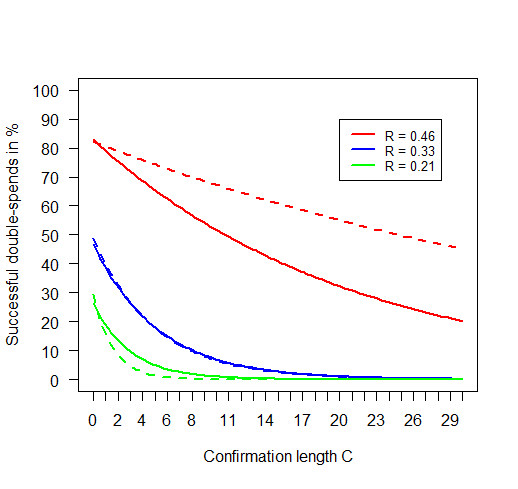
\includegraphics[width=\linewidth]{Comparison/Confirmations/conf.png}
\end{subfigure}
\begin{subfigure}{.495\textwidth}
  \centering
  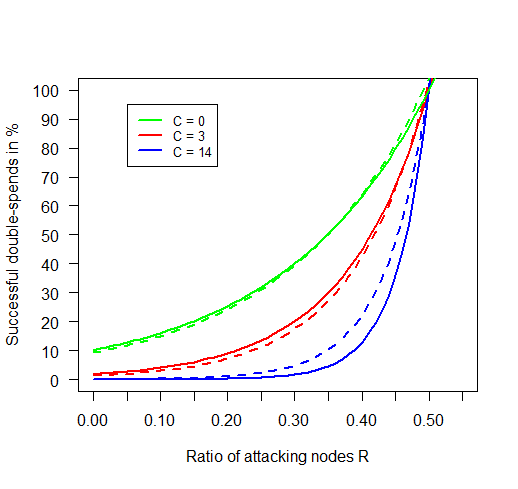
\includegraphics[width=\linewidth]{Comparison/Confirmations/confrat.png}
\end{subfigure}
\begin{subfigure}{.495\textwidth}
  \centering
  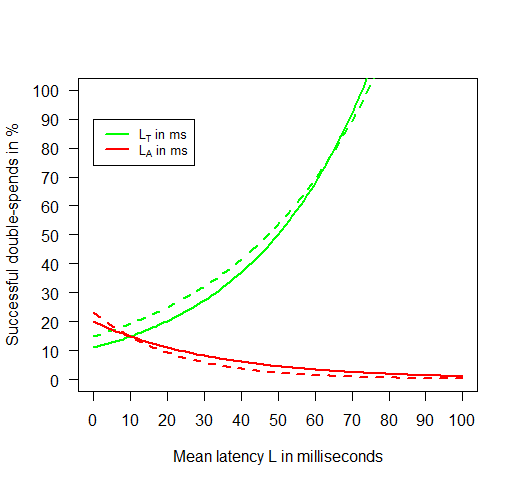
\includegraphics[width=\linewidth]{Comparison/bothlat.png}
\end{subfigure}%
\begin{subfigure}{.495\textwidth}
  \centering
  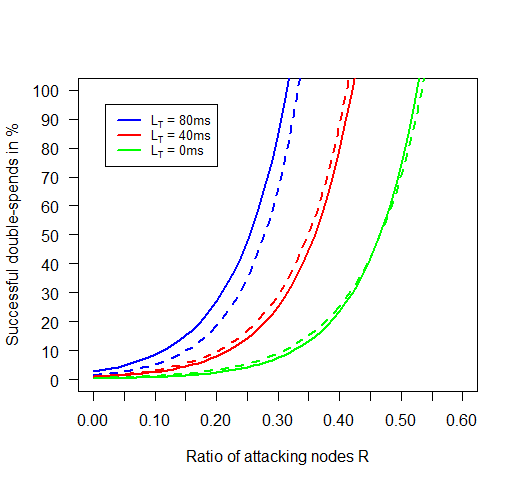
\includegraphics[width=\linewidth]{Comparison/TruLatency/trurat.png}
\end{subfigure}
\begin{subfigure}{.495\textwidth}
  \centering
  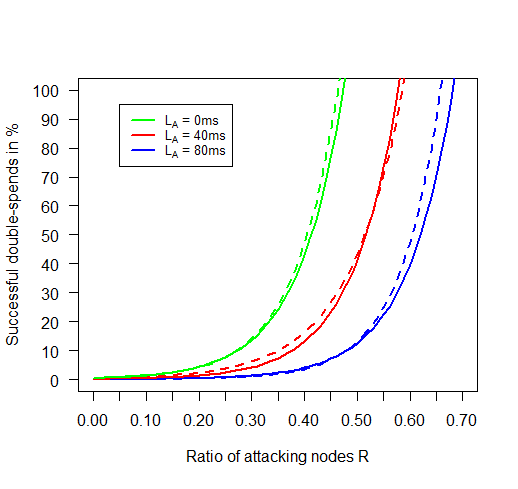
\includegraphics[width=\linewidth]{Comparison/AttLatency/attrat.png}
\end{subfigure}
\begin{subfigure}{.495\textwidth}
  \centering
  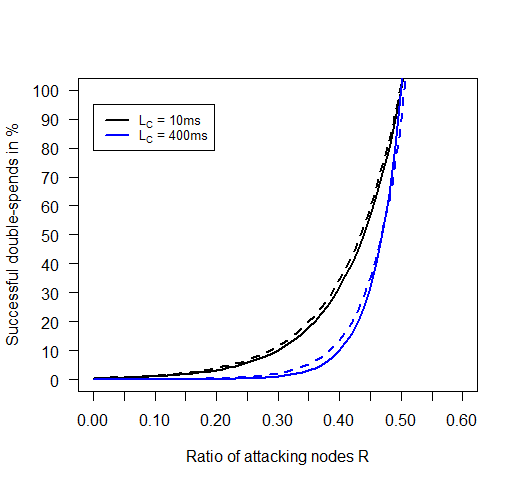
\includegraphics[width=\linewidth]{Comparison/ConnLatency/conrat.png}
\end{subfigure}
\caption{Comparison of fitted curves and the proposed model}
\label{comp}
\end{figure}

\begin{figure}
\centering
\begin{subfigure}{.495\textwidth}
  \centering
  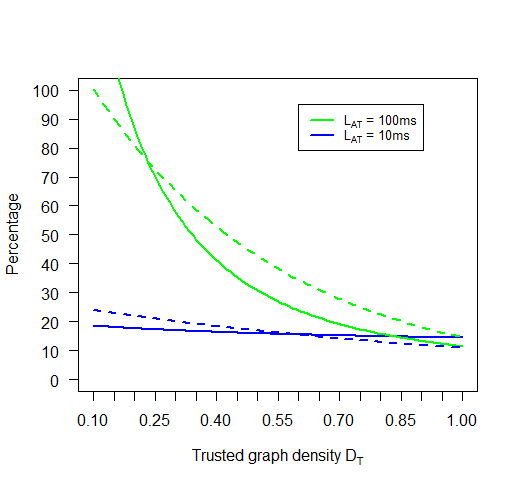
\includegraphics[width=\linewidth]{Comparison/TruDensity/trudens.png}
\end{subfigure}
\begin{subfigure}{.495\textwidth}
  \centering
  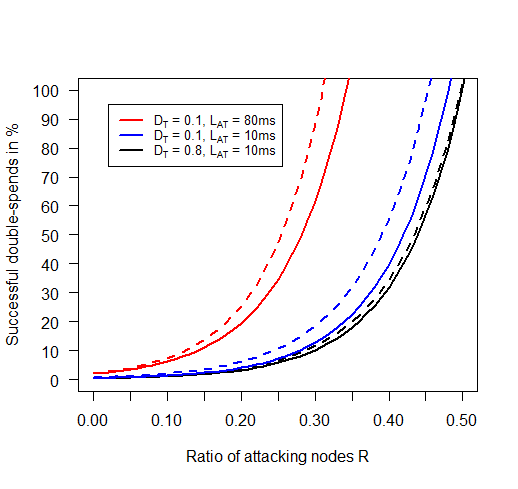
\includegraphics[width=\linewidth]{Comparison/TruDensity/trudensrat.png}
\end{subfigure}
\begin{subfigure}{.495\textwidth}
  \centering
  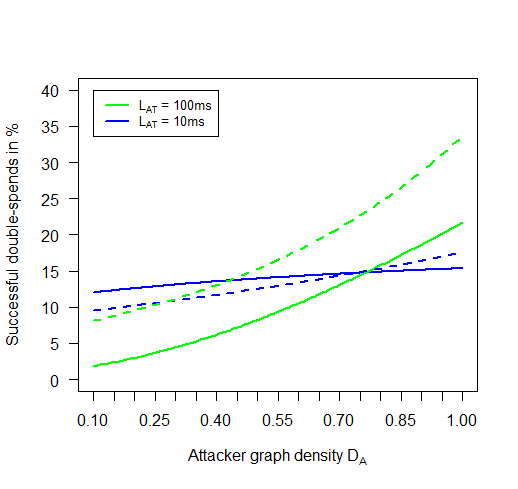
\includegraphics[width=\linewidth]{Comparison/AttDensity/attdens.png}
\end{subfigure}%
\begin{subfigure}{.495\textwidth}
  \centering
  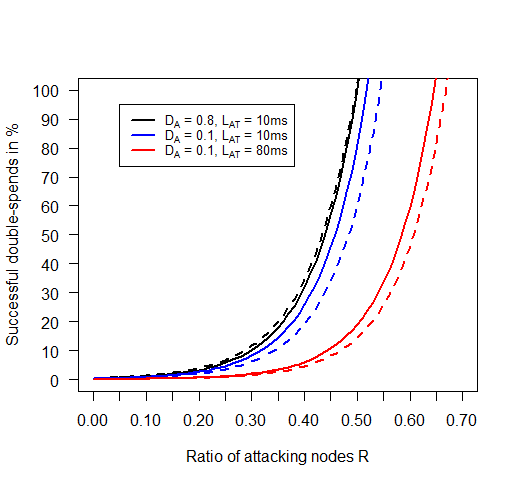
\includegraphics[width=\linewidth]{Comparison/AttDensity/attdensrat.png}
\end{subfigure}
\begin{subfigure}{.495\textwidth}
  \centering
  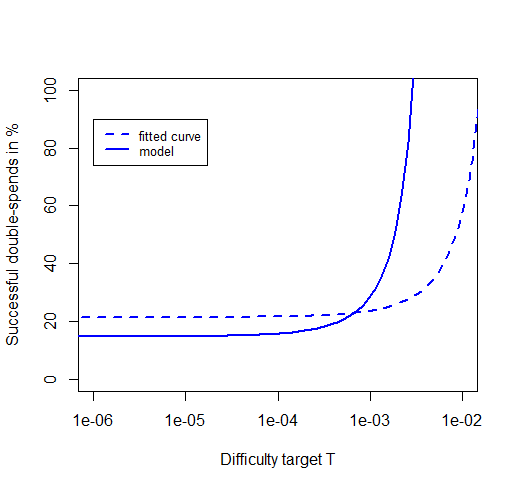
\includegraphics[width=\linewidth]{Comparison/Difficulty/difficultyfit.png}
\end{subfigure}
\begin{subfigure}{.495\textwidth}
  \centering
  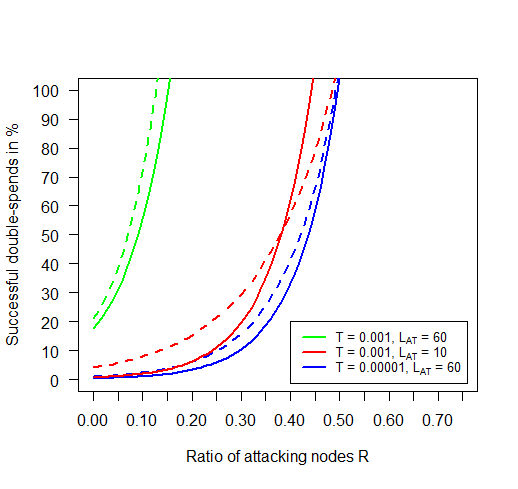
\includegraphics[width=\linewidth]{Comparison/Difficulty/diffrat.png}
\end{subfigure}
\caption{Comparison of fitted curves and the proposed model}
\label{comp2}
\end{figure}
\subsection{Discussion} \label{modeldisc}
Although our model is not entirely accurate, the general profile of the plotted formula matches the individually fitted curves of the data. Some loss of precision can be explained by the chosen experimental design of Section \ref{design}. During the experiments, most parameters were set to the default configuration of Appendix \ref{defaultval}. Since our model is ultimately fitted to the data generated by the experiments, the formula is expected to be especially accurate as long as the applied parameters are close to the default configuration. Moving further away from this configuration consequently reduces the precision of our model, resulting in effects similar to the red curves in the first plot of \autoref{comp}. 

\section{Limitations} \label{modellimit}
Next to the limitations of Section \ref{limits} which ultimately reflect on the model and the inaccuracies discussed in sections \ref{modelcomp} and \ref{modeldisc}, some further threats to the validity of our proposed formula can be identified. 

Firstly, there might be additional factors affecting the RADS of a block-chain architecture which are missing in the implementation of our simulator and are consequently not included in the model definition. One of these potentially missing factors is the connection density $D_C$ already mentioned in Section \ref{limits}. This parameter could lead to an amplifying effect on $L_C$, similar to the observed relation between $D_T$ and $L_T$ ($D_A$ and $L_A$). A second parameter not included in the simulator and the model is the amount of lost block transmissions due to packet loss. This phenomenon is present in real blockchain architectures and leads to missing blocks and the generation of orphan blocks (Section \ref{peer2peer}) in the networks. A node is unable to mine on top of a received orphan block as these blocks are disconnected from the local blockchain copy. Therefore, a potentially longer blockchain might remain unknown to the node until all missing parent blocks are acquired. In the mean time, the node persists on mining on the valid, shorter blockchain. If blocks mined onto this shorter chain are then replaced by the orphan block and its delayed parents, the number of generated stale blocks increases. Since the number of stale blocks has an effect on $PDS$ (as shown in Section \ref{discussion}), a packet loss parameter could influence a blockchain architecture's RADS. Simulating this parameter would require implementing the transmission of single blocks in our simulator, as opposed to the current propagation of whole blockchain copies.


Similar to missing parameters, the relationships between parameters pre-sent another threat to our model. Although relationships between the latency, density and difficulty parameters have been identified, their modeling in Section \ref{building} might be inaccurate. Furthermore, the existence of additional relationships which are not yet modeled by our formula should be considered. 

Lastly, the model's empirical constants (\autoref{constants}) were iteratively fitted to the experimental data using non-linear regressions \cite{nlxb}. These constants might be erroneous and rely fundamentally on the quality and amount of the sampled data they are fitted to.

Nevertheless, the model presents a good estimate of the simulator's results. It can be used to make predictions regarding the RADS of a blockchain architecture without explicitly running the simulator and enables additional mathematical methods of analyzing the resistance against double-spend attacks, for example solving the equation for different model parameters. Overall, the formula provides an adequate starting point for further refinement, which includes the identification and incorporation of missing factors and relationships, as well as improving the fitting of our empirical constants.
%------- chapter 7 -------

\chapter{Conclusion} \label{conclusion}
\begin{sloppypar} In this thesis we analyzed the resistance of blockchain architectures against double-spend attacks (RADS) using simulation and experimentation. Since existing work regarding RADS is primarily focused around simplified mathematical models, the goal was to improve an architect's predictions of a blockchain's RADS, based on empirical parameters inspired by real blockchain protocols. Our objectives were the identification and evaluation of factors affecting a blockchain architecture's RADS, the implementation of a blockchain simulator to provide evidence on the parameters' effects and the formulation of an empirical model based on the simulator's results. \end{sloppypar}
\section{Summary}
Chapter \ref{intro} provided an introduction to the topic. We gave a definition of the problem statement leading to our objectives and formulated our intended approach. 

In Chapter \ref{background} we described the general concept of blockchain architectures and networks, using Bitcoin as a concrete example of application. We presented the chaining of blocks through hashing combined with the proof of work algorithm as a persistent way of securing consensus and integrity of data. We discovered the natural generation of stale blocks and branches in a network influenced by propagation delays and presented the longest chain rule as the central mechanism to regain consensus. Lastly, we introduced double-spend attacks and their potential to maliciously break blockchain protocols. We described an attacker \textit{A} capitalizing on a target merchant \textit{M} who is only waiting for a set amount of confirmations before sending the purchased products. By secretly mining a longer blockchain branch than the remaining network, \textit{A} was able to modify the initial transaction paying the merchant to a self-receiving transaction. \textit{A} thereby received the purchased product and reverted the payment.

Chapter \ref{relatedwork} provided a survey of related work regarding mathematical and empirical models of RADS, while also considering other attacks on blockchains similar to DSA. We stated our contribution to the topic and identified parameters relevant to our investigations. Included in these parameters were the number of attacking and trusted nodes, the network topology and latency, the number of confirmations required by the targeted merchant and the mining difficulty representing the maximum value of a valid proof of work. 

In Chapter \ref{simulator} we presented our blockchain simulator developed to experiment the effects of these parameters on RADS. After describing the general architecture and components of the simulator framework, we presented different strategies of modeling a peer-to-peer network of nodes. We subsequently used the framework to implement a simulation of double-spend attacks by extending the frameworks functionality. The simulation was modeled by defining a network of attacking nodes conducting the double-spend attacks and a network of trusted nodes adhering to the simple protocol of mining on the longest chain they are aware of. The topologies of both networks were simulated according to parameters defining the density and mean latency of the underlying graphs.

Chapter \ref{eval} made use of the implemented simulator by conducting several experiments of different parameter configurations. By measuring the percentage of successful double-spend attacks ($PDS$) during each simulation run, a range of data samples was created describing the effects of each parameter. The significance of these effects was tested using the Kruskal-Wallis hypothesis test \cite{kruskal,r}, computing 95\% confidence levels for each parameter. Next to $PDS$, a second focus was set on analyzing the parameters' effects on the percentage of stale blocks mined by the attacking ($PSB_A$) and trusted ($PSB_T$) networks. Stale blocks are created when two blocks are mined onto the same parent block as a result of propagation delay. Therefore, stale blocks create a fork of the blockchain, which is eventually resolved by the longest chain rule. When evaluating double-spend attacks, these blocks consequently do not contribute to the length of trusted and attacking blockchains, indicating a ``waste'' of computing power. Overall, the most important results of our experiments can be summarized as follows:
\begin{itemize}
\item Similar to \cite{nakamoto2008bitcoin,HBDSA,DSAwithTime}, the $PDS$ increases exponentially with increasing hashing power (nodes) controlled by the attacker.
\item However, only considering the distribution of hashing power is insufficient. Instead, $PDS$ depends on the distribution of \textit{effective} computing power available to both networks.
\item \textit{Effective} computing power depends on the amount of computation being ``wasted'' towards the creation of stale blocks which are not part of the valid blockchain.
\item The amount of stale blocks created by a network is influenced by the latency and density between its peers, as well as the mining difficulty.
\item High latencies and a low network density increase the time needed for a block to reach all nodes. This increases the chance of stale blocks and therefore the amount of wasted computing power.
\item Low difficulty targets result in less blocks being mined overall. By maximizing the average time between the creation of blocks, chances of two nodes mining blocks at roughly the same time decrease. Therefore, the amount of wasted stale blocks is minimized.
\item Similar to \cite{HBDSA}, the $PDS$ decreases exponentially with increasing confirmation length.
\end{itemize}
Concluding the evaluation, we described limitations of our results, especially concerning the implementation of the simulator and the missing in-depth hypothesis testing. 

Chapter \ref{modelchapter} used the achieved results and the generated simulation data to formulate an empirical model indicative of our simulator's RADS for different parameter configurations. The model was formulated by creating a simple exponential model of a single parameter and iteratively including additional parameters. The occurring undefined constants were fitted to the simulator's data using non-linear regressions during each iteration step. The resulting formula was subsequently compared to all individually fitted curves describing the experiments of Chapter \ref{eval}. Following this comparison, potentially missing parameters and other causes for the observed precision loss were identified. 
\subsection{Realized Goals}
We successfully identified eight parameters affecting a blockchain architecture's RADS. By implementing a simulator of double-spend attacks, the effects of all parameters were evaluated empirically. The statistical significance of each parameter was confirmed by Kruskal-Wallis tests computing 95\% confidence levels. Lastly, we successfully proposed an empirical model based on experimental data, representing the effects of all parameters (\autoref{formula}). 
%The evaluated parameters are specifically:
%\begin{itemize}
%\item The ratio of attacking nodes $R$.
%\item The number of confirmations $C$ required by the targeted entity relying on the altered block's data.
%\item The attackers' ability to publish fraudulent blockchains defined by the latency $L_C$.
%\item The latency between peers of the attacking ($L_A$) and trusted ($L_T$) networks.
%\item The density of attacking ($D_A$) and trusted ($D_T$) networks.
%\item The mining difficulty target $T$.
%\end{itemize}
\subsection{Open Goals}
Our open goals can be described by summarizing the limitations identified in Section \ref{limits}. The underlying model of our double-spend simulator is simplifying some aspects of real blockchain architectures, despite our goal of simulating double-send attacks realistically. Firstly, by propagating whole blockchain copies instead of single blocks, possible effects of packet loss and orphan blocks are disregarded. Secondly, as explained in Section \ref{limits}, the creation of peer-to-peer networks is not perfectly random. Thirdly, the abstract \textit{ConnectionStrategy} (Section \ref{connstrat}) modeling an attacker's ability of publishing secret blockchain branches, is missing additional, more realistic implementations. Furthermore, the Kruskal-Wallis tests used to determine the significance of our parameters are usually followed up by post-hoc tests in order to identify the specific treatment levels leading to the observed effects. However, such a test was not conducted in the context of this thesis.
\section{Implications}
Summarizing our results, the definition of double-spend attacks as 51\% or majority attacks is misleading. Despite an attacker controlling more than 50\% of the total hashing power, double-spend attacks are not necessarily guaranteed, since the effective value of attacking nodes might be decreased by high block propagation delays. On a similar note, double-spend attacks with less than 50\% hashing power controlled by an attacker might be more likely than originally anticipated, if conducted by a network mining at very high efficiency (see figures \ref{latplot} and \ref{densplot}). Overall, the hashing power of a blockchain network should always be regarded in relation to the mining efficiency, which depends on the amount of computing power being wasted towards the generation of stale blocks.

According to \cite{infoprop}, the Bitcoin architecture only experiences an average of 1.69\% stale blocks. The difficulty target chosen by Bitcoin is therefore sufficiently low in order to offset the effects of block propagation delay. Nevertheless, as shown by our results, blockchain architectures with higher rates of stale blocks are more vulnerable to double-spend attacks. In this regard it is important to note that the amount of stale blocks might be increased by potential denial-of-service attacks targeting the communication between nodes.

Fulfilling our objective for this thesis, the implemented double-spend simulator and our proposed empirical model can be used by an architect to make predictions about a blockchain architecture's RADS. After specifying a parameter configuration describing the architecture, simulator and model both return the percentage of successful double-spend attacks ($PDS$) which is indicative of a blockchain's RADS. The model can additionally be used as a starting point for further mathematical analysis of RADS.
\section{Future Work}
Although our simulator and model represent an empirical improvement over mathematical models only considering the distribution of pure hashing power and the confirmation length, there might still be parameters missing in our investigations, whose effects on RADS remain unknown. Potential candidates for these parameters are mentioned in Section \ref{modellimit}. Looking forward, concrete missing factors should be identified and included in our simulator and model.

As seen in Section \ref{modeldisc}, our proposed model is not entirely accurate and is fitted to data mostly depending on the default configuration of Appendix \ref{defaultval}. Therefore, the precision of our model could be improved by performing additional experiments and simulation runs, while making use of extensive and more elaborate regression techniques.

Using our results, the potential threat of double-spend attacks could be revisited. This could be done by investigating the game theoretical economics of double-spend attacks on real world blockchains, for example the Bitcoin protocol, while also considering the possible influence of attackers on the honest nodes' network topology.

The insights of this thesis and the developed simulation framework open up additional possibilities of further investigations and analysis of blockchain architectures. By comparing our results to the hashrate-based models mentioned in Chapter \ref{relatedwork} or performing additional simulation runs suited to those models, the mathematical formulas could be validated by empirical data or possible flaws could be discovered. On a similar note, the simulation framework could be used to implement and evaluate other attacks on blockchains, for example the \textit{selfish-mine} attack mentioned in Section \ref{otherattacks}. This would allow further investigations of blockchain architectures, comparable to our thesis on double-spend attacks. 



\appendix

\chapter{Property Files} \label{prop}
Property files can be used to permanently store parameters and allow simple configuration of the simulated conditions. The property file's structure is a list of key-value pairs, defined as an assignment of values to parameter names (keys) as shown in \autoref{propstruc}. In the following a short summary of all available parameters and possible values will be presented.
\begin{lstlisting}[caption=Property file structure,label=propstruc]
<parameter1> = <value1>
<parameter2> = <value2>
...
\end{lstlisting}
\subsubsection{NUM\_TRUSTED, NUM\_ATTACKER}
The number of honest and attacking miners in the simulated network should be greater than zero. Since each node corresponds to an additional program thread, higher numbers of nodes should be considered carefully.
\subsubsection{DIFFICULTY}
The difficulty target of mining a block. The parameter should be specified as a floating point number between 0 and 1.
\subsubsection{CONFIRMATIONS}
The number of blocks required by the targeted merchant to consider a transaction as confirmed should be non-negative.
\subsubsection{LAT\_TRUSTED, LAT\_ATTACKER}
The mean latency in milliseconds used to create the Gaussian distribution presented in Section \ref{distribution} should be non-negative. Parameters for trusted and attacking networks can be defined individually to allow simulation of different connection qualities in the networks.
\subsubsection{LAT\_CONNECTION}
The mean latency in milliseconds used to model the connection between attacking and trusted network is non-negative. It simulates the attackers' ability of publishing fraudulent branches to the honest network.
\subsubsection{DENS\_TRUSTED, DENS\_ATTACKER}
The graph density of the attacking and trusted networks as defined by the \hyperref[rndgraphstrategy]{\textit{RndGraphStrategy}}. Since the created graph has to be connected, the specified floating point value should be in the range of $[\frac{2}{n}, 1]$, where $n$ is the number of nodes in the graph.
\subsubsection{RUNS}
The number of double-spend attempts carried out by the Simulator for each simulation.
\subsubsection{EPSILON}
The fault tolerance corresponding to Section \ref{faulttolerance} should be a floating point value in the range of $(0, 1)$.
\subsubsection{LOGGING}
Controls the amount of console output. Possible values are \textit{INFO}, \textit{FINE}, \textit{FINER}, \textit{FINEST}, whereas the amount of detail corresponds to $\textit{INFO} < \textit{FINE} < \textit{FINER} < \textit{FINEST}$.
\subsubsection{PS\_TRUSTED, PS\_ATTACKER}
These parameters can be set to select the peer strategies used to create the networks. Strategies requiring the definition of an adjacency matrix cannot be specified using property files. Possible values are therefore: \textit{CONSTANT}, \textit{EUCLIDEAN}, \textit{RANDOM}, referring to the strategies defined in Section \ref{peerstratsection}.
\subsubsection{CONN\_STRAT}
This parameter can be set to select the connection strategies used to create a link between attacking and trusted network. Currently the only possible value is \textit{CONSTANT}.
\subsubsection{Randomized Parameters}
Bounds of randomized parameters can be specified by providing the inclusive lower and upper bounds, where $lower < upper$ (\autoref{boundstruc}). If bounds of a parameter have been specified by the loaded property file, the parameter will automatically be randomized during the simulation after each double-spend attempt. Randomizable parameters are latencies, graph densities and the number of confirmations.
\begin{lstlisting}[caption=Defining bounds of randomized parameters,label=boundstruc]
<parameter1_BOUNDS> = <lower1>, <upper1>
<parameter2_BOUNDS> = <lower2>, <upper2>
...
\end{lstlisting}
\subsubsection{Default Values}\label{defaultval}
Undefined parameters will be initialised with default values as defined in \autoref{default}. 
\begin{lstlisting}[caption=Default parameter values,label=default]
NUM_TRUSTED    = 32
NUM_ATTACKER   = 16
DIFFICULTY     = 0.00001
CONFIRMATIONS  = 6
LAT_TRUSTED    = 10
LAT_ATTACKER   = 10
LAT_CONNECTION = 10
DENS_TRUSTED   = 0.8
DENS_ATTACKER  = 0.8
RUNS           = 100
EPSILON        = 0.00001
LOGGING        = FINE
PS_TRUSTED     = RANDOM
PS_ATTACKER    = RANDOM
CONN_STRAT     = CONSTANT
\end{lstlisting}

\chapter{Model Parameters} \label{modelparams}
\begin{table*}[ht]
\centering
\begin{tabular}{|l|l|l|l|l|}
\hline
Figure & Subfig. & Curve & A & B \\ \hline
\ref{ratio}					&					   & blue & 0.440456 & 10.901 \\ \hline
\multirow{5}{*}{\ref{conf}} & \multirow{3}{*}{(a)} & red & 82.1968 & -0.0200805 \\
 							& 					   & blue & 48.9006 & -0.201187 \\
 							& 					   & green & 29.4556 & -0.621696 \\ \cline{2-5}	
 							& \multirow{2}{*}{(b)} & green & 9.19904 & 4.8539 \\
 							&					   & red & 1.21852 & 8.87987 \\
 							& 					   & blue & 0.0521142 & 15.1466 \\ \hline
\multirow{2}{*}{\ref{conn}} & (a) & blue & 15.5299 & -0.00498 \\ \cline{2-5}	
 							& (b) & blue & 0.00721199 & 18.8602 \\ \hline
\multirow{8}{*}{\ref{latplot}} & (a)				   & blue & 14.9187 & 0.0255749 \\ \cline{2-5}	
 							& \multirow{3}{*}{(b)} & blue & 1.473 & 12.675 \\
 							& 					   & red & 1.07143 & 11.0149 \\ 
 							& 					   & green & 0.420428 & 10.2444 \\ \cline{2-5}	
							& (c)				   & blue & 23.3313 & -0.0461159 \\ \cline{2-5}	
 							& \multirow{3}{*}{(d)} & green & 0.378158 & 12.0494 \\
 							& 					   & red & 0.327956 & 9.76266 \\ 
 							& 					   & blue & 0.0214614 & 12.8297 \\ \hline
\end{tabular}
\end{table*}
\begin{table}[tp]
\centering
\begin{tabular}{|l|l|l|l|l|}
\hline
Figure & Subfig. & Curve & A & B \\ \hline
\multirow{8}{*}{\ref{densplot}} & \multirow{2}{*}{(a)} & green & 124.344 & -2.14213 \\
 							& 					   & blue & 26.2039 & -0.88155 \\ \cline{2-5}	
 							& \multirow{2}{*}{(b)} & red & 2.12947 & 12.394 \\ 
 							& 				       & blue & 0.678576 & 11.0063 \\ \cline{2-5}
							& \multirow{2}{*}{(c)} & green & 6.9238 & 1.58297 \\
 							& 					   & blue & 8.88541 & 0.68364 \\ \cline{2-5}	
 							& \multirow{2}{*}{(d)} & blue & 0.20031 & 11.4103 \\ 
 							&    				   & red & 0.0459435 & 11.5084 \\ \hline
\multirow{4}{*}{\ref{diff}} & (a)				   & blue & 21.5139 & 99.4238 \\ \cline{2-5}	
 							& \multirow{3}{*}{(b)} & green & 20.947 & 12.2793 \\
 							& 					   & red & 4.11228 & 6.57397 \\ 
 							& 					   & blue & 0.905035 & 9.54316 \\ \hline
\end{tabular}
\caption{Parameters of fitted curves in Section \ref{results}}
\end{table}





\clearpage

\listoffigures
\clearpage

\listoftables
\clearpage

\bibliography{thesis}
\bibliographystyle{alpha}

\end{document}
